\startchapter{Empirical Application}
\label{chapter:Exp}

In this chapter, we  report our results from an empirical application. We use five economic variables to predict GDP for Canada. 

\section{Why Choose Financial Data?}


\citeA{Andreou2013a} demonstrate that daily financial data can help forecast and nowcast the quarterly real GDP growth.  \citeA{BANBURA2014} show that real time daily financial data can improve the nowcasting of low frequency macroeconomic data.  \citeA{Ferrara2013}  have recently shown that  daily financial series have a significant forecasting power when it comes to  US economic growth, specially when the volatility of those signals is considered as a explaining factor and not only its returns. 


We choose real gross domestic product(GDP) for Canada as the target variable for forecasting. GDP is a very important indicator for economic activity and has been used for economic decisions and public policy in many institutions. Forecasting GDP is very challenging since it is related to and affects many factors such as employment, consumption, and  exports. In this chapter, we show BSTS-U-MIDAS can help to improve forecast accuracy, compared to ARIMA model. In practice, AR(1) and AR(4) models perform very well, and a few models can outperform them \cite{Koopman2013}. Our empirical evidence shows that a BSTS-U-MIDAS model performs very well during the 2007-2011 financial crisis period. It shows that BSTS-U-MIDAS model is more capable to predict the change points and structural breaks.     





\section{Data}

We choose 5 macroeconomic variables in the regression component of our model. They are daily Toronto Stock Exchange (TSX) index and West Texas crude oil prices, monthly unemployment rate, spread between interest rates of ten years government bonds and three month treasure bill , and  housing starts data. Those variable are high correlated with Canadian GDP. (Details of the data are discussed in Appendix B)

The data of real GDP for Canada and housing starts are taken from Statistics Canada. The data of the monthly unemployment rate,  spread between interest rates of 10 years government bonds and treasure bill , and   West Texas crude oil prices are taken from FRED® database. TSX composite index is taken from Yahoo finance. 

We estimate three models with different sets of data. The first model has  monthly unemployment rate, spread between interest rates of 10 years government bonds and treasure bill, and TSX composite index. The second model has housing start and the data in first model. The third model has West Texas crude oil prices and the data in second model. In this section we are going to discuss the details for third model and some remarkable differences between the three models. (See the details for the first and second models in Appendix C.)  



\subsection{Target: GDP growth rate for Canada}



Our target variable is the growth rate of total gross domestic product for Canada. It is a quarterly ,seasonally adjusted data which is measured by expenditure in constant prices. Figure ~\ref{fig:gdp-growth} shows the dynamics of GDP growth for Canada between 1980 and 2015.

%\begin{figure}[h]
%\centering
%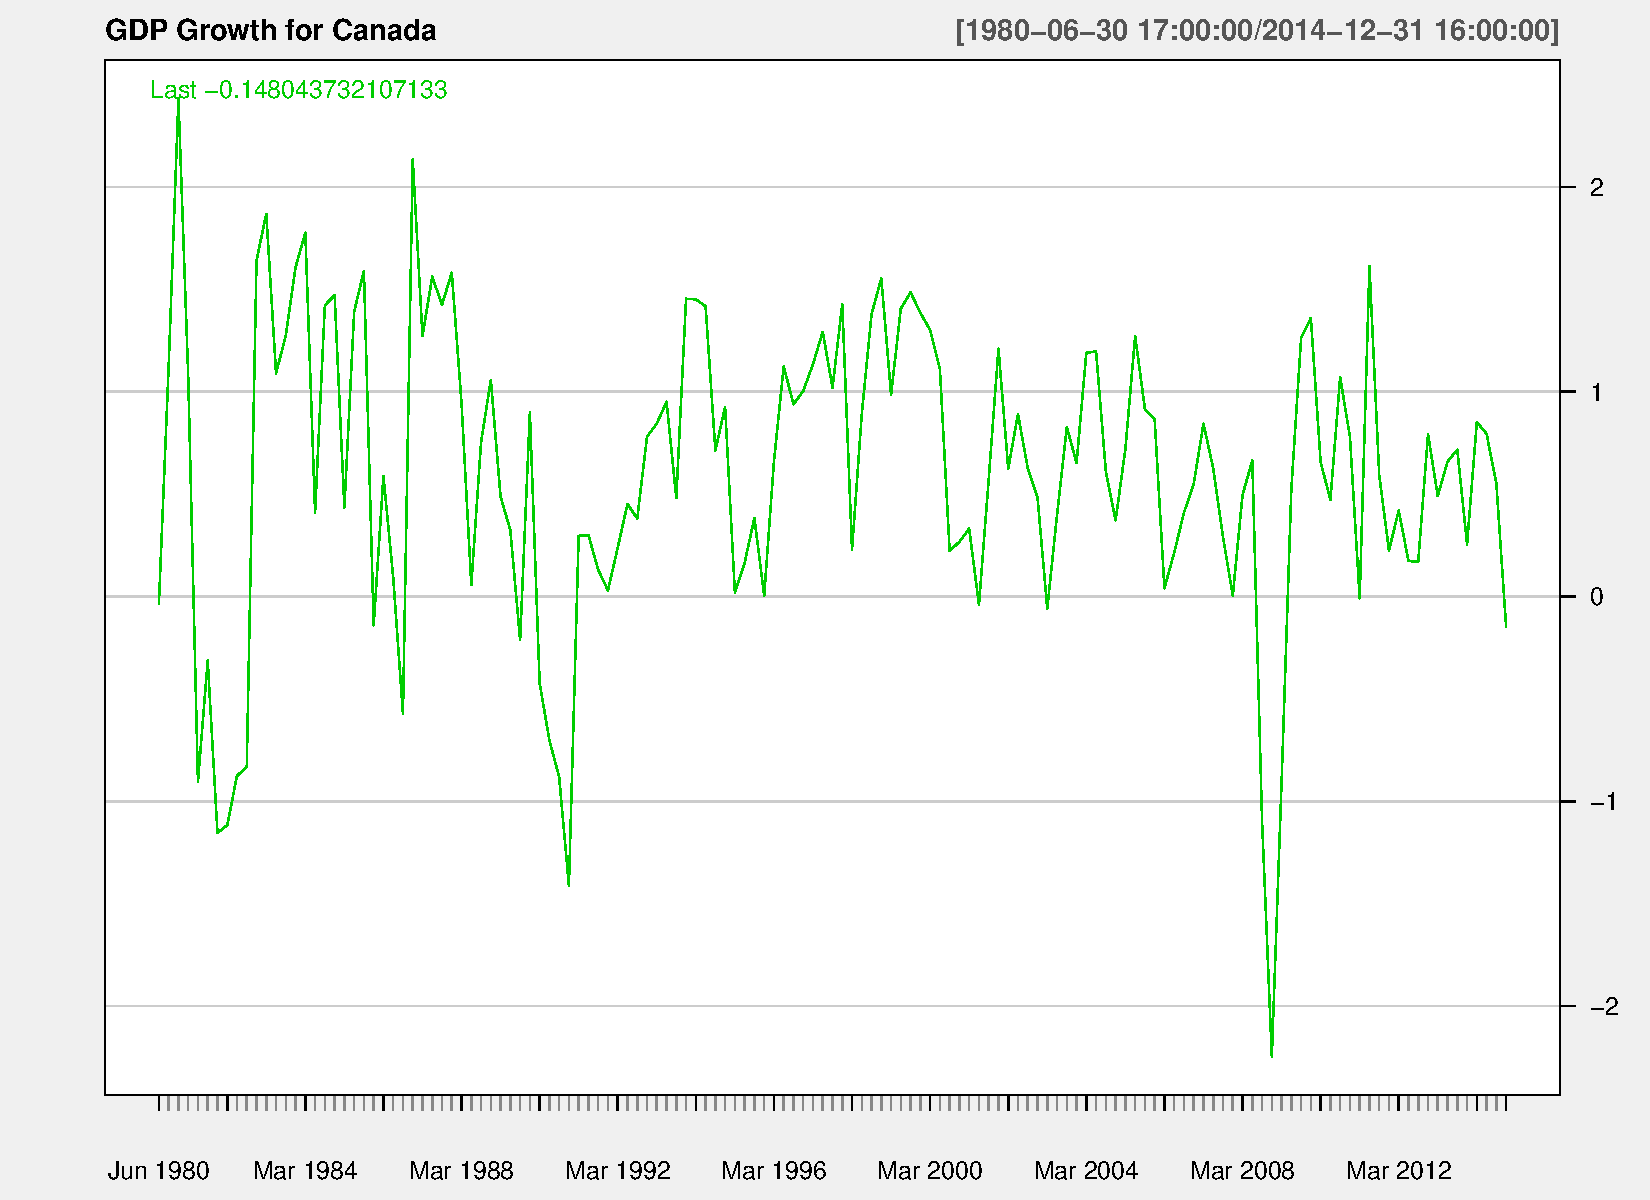
\includegraphics[width=0.6\linewidth]{Figures/gdp-growth-report}
%\caption{GDP for Canada 1980/07-2015/01 Quarterly}
%\label{fig:gdp-growth}
%\end{figure}

In order to compare performance of BSTS, ARIMA and Boosting models, we need a stationary time series data for the ARIMA, so we calculate GDP growth rate by   differencing log GDP. The log differenced GDP passes the unit root and stationary test at 5\% significance level.  



\begin{figure}[h]
	\centering
	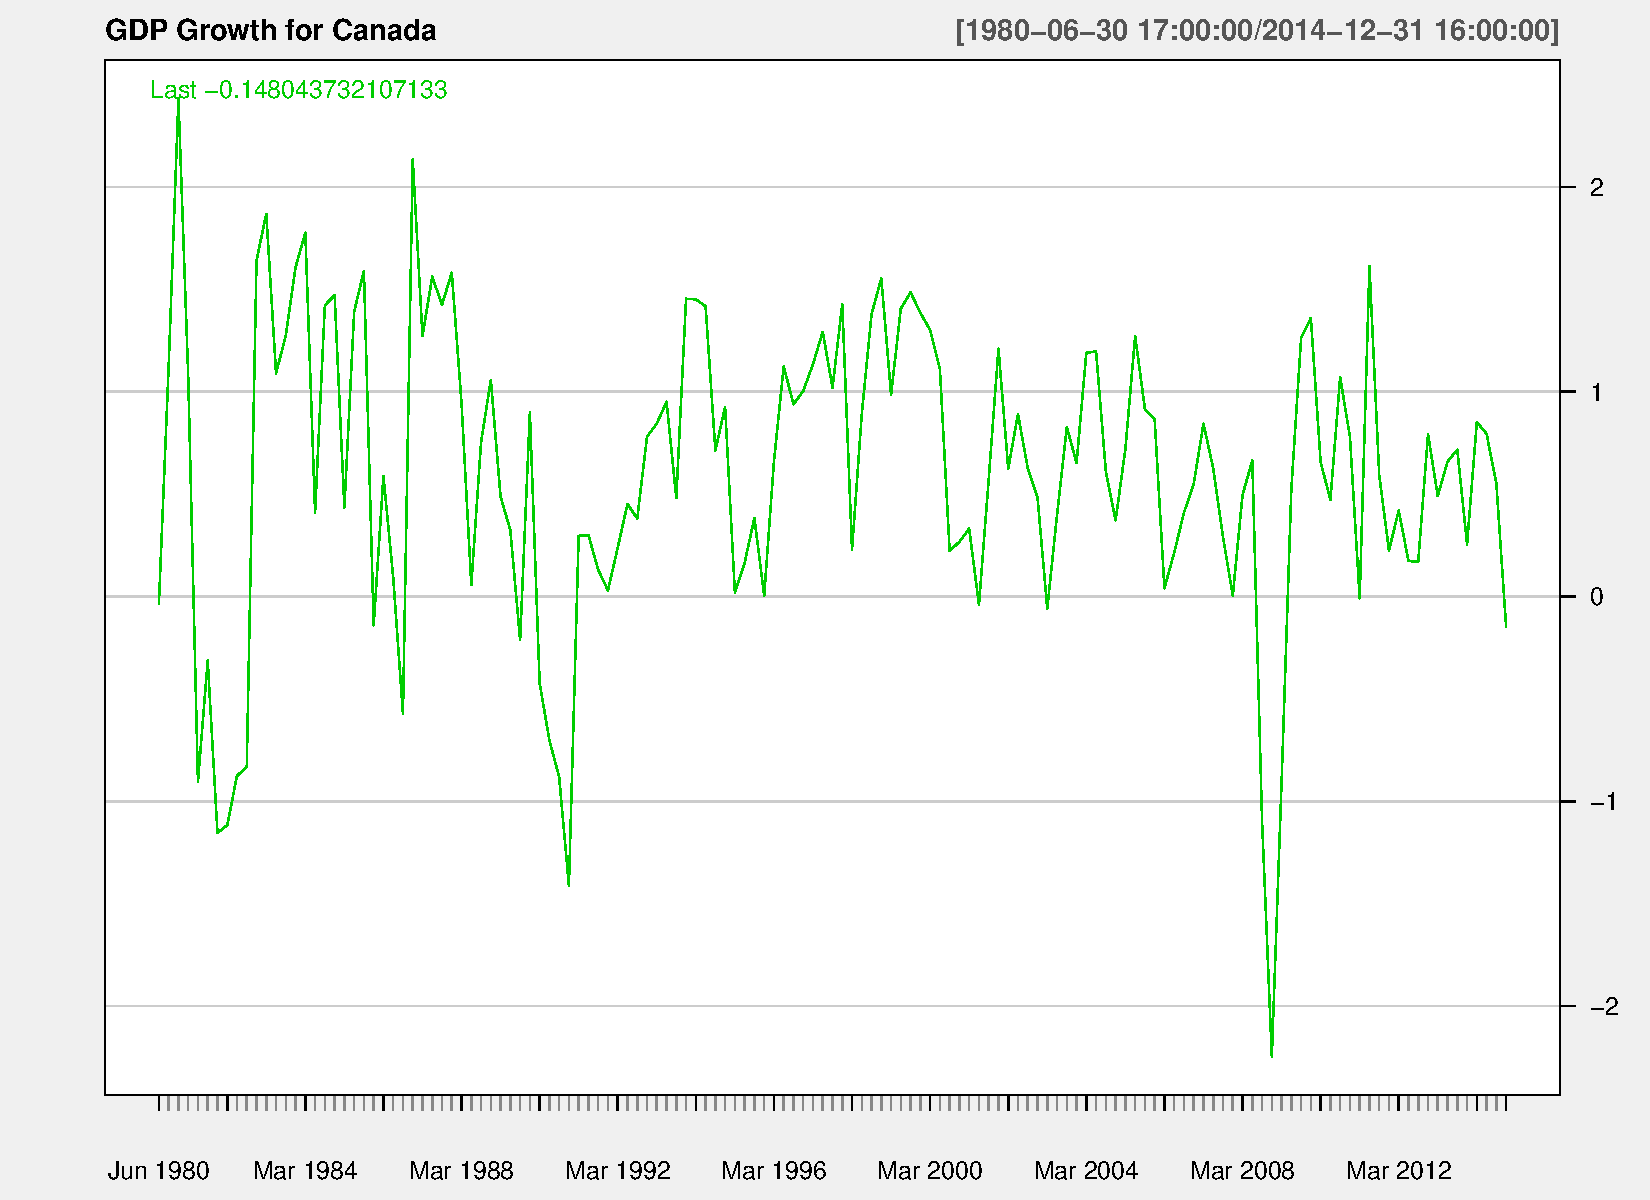
\includegraphics[width=0.6\linewidth]{Figures/gdp-growth-report}
	\caption{Real GDP Growth Rate (percent)  for Canada 1980/07-2015/01 Quarterly}
	\label{fig:gdp-growth}
\end{figure}


 


\subsection{Pre-process of the data: whiten data}



As we have mentioned, all predictors' data are realigned to match up to the quarterly frequency by the skip-sampled method that we discuss in the previous chapter. All predictors' information is given in  Appendix B. 

Due to the data availability, we match up all data at a window between 1980 third quarter and 2015 first quarter by using the MIDAS (mixed-data sampling) method in first and second models. The third model has the data at a window between 1986 fourth quarter and 2015 first quarter since we only have West Texas crude oil prices data down to 1986 fourth quarter. After a MIDAS skip-sampled transformation, each monthly time series data becomes a matrix with 3 quarterly time series data components, and each daily time series data becomes a matrix with $22 \times 3 $ time series data components.



The data set is ragged. Different time series data have different the most recent data point. For example, for the daily data such as the TSX composite index, we choose the data up to May 28. Since Statistics Canada publishes the first quarter's GDP data on May 29, 2015, we are able to keep updating our forecasting practice using daily data until May 28, 2015. In terms of monthly data, we are able to include data up to March 2015.  

For all predictors, we  include leads and lags in the regression. For  monthly data, we keep 23 month lags (two years). For  daily data, we keep $12 \times 22-1$ lags (one year). Then in the third model, the total number of predictors in the regression component is $600$, but we only have 114 observations. Our model is a fat regression type model. Our BSTS-U-MIDAS model does not select some specific variables. Instead, it calculates the probability of inclusion of variables and compute the posterior distribution of the prediction.

In order to avoid spurious regression, we detrend, deseasonalize, and scale the predictors using the ``decomp" command in R package ``forecast" \cite{Hyndman2015}. The target variable is seasonally adjusted. We also deseasonalize the target variable since in our case, deseasonalizing target variable improve the forecasting performance. For daily data such as TSX index and oil price, we also take first order log difference to obtain stationarity, so in some sense, the returns of TSX index and oil price are included in the models. 

The rationale behind pre-processing data is to avoid the spurious regression \cite{Scott2014a}. Without the common trend and seasonality, the variation of the target variable can be more accurately estimated by the variation of the predictors.  

\section{Results: One Period Ahead Forecasting / Nowcasting}


In our application, we use a generalized local trend model with AR(4) component and a regression component with 10000 MCMC iterations  and 2000 burn-in. (See Appendix C for details). We add AR terms of target variable in the model in order to utilize the information of lagged target variables for forecasting. For simplicity, we include AR terms up to AR(4) since our target variable is quarterly data. 

In a state-space presentation of BSTS-U-MIDAS model, the expected filtered ``observation" is one period ahead forecast, which is estimated by the predicted state plus regression component. 

$$gdp_{t} = F_{t}\alpha_{t}+ z_{t} +v_{t},\quad  v_{t}\sim \mathcal NID(0,V_{t})$$


$$\alpha_{t} = G_{t}\alpha_{t-1}+w_{t},\quad  w_{t}\sim \mathcal NID(0,W_{t})$$

Let $ GDP^t = (gdp_1, ..., gdp_t) $ be the vector of observation up to time t. The \textit{filtering} distributions, $p(\alpha_t|GDP^{t}) $ can be computed recursively as follows, where $\alpha$ denotes the states which includes trend and AR term in our time structural model.:

First, we start with initial value $ \alpha_0 \sim N(m_0, C_0) $ at time $0$. Then we enter a prediction stage and  estimate the one step forecast for the \textit{state}: 
$$\hat{\alpha_t}|GDP^{t-1} \sim N(a_t, R_t) $$
where $a_t = G_t \cdot m_{t-1}$ , and $R_t = G_t C_{t-1} G_t^\prime + W_t$. In our BSTS model,  $G_t$ is the transition or system matrix. (The details are discussed in Appendices A and C)  



\subsection{Distribution of one step ahead forecast for observations}

One step forecast for the \textit{observation} can be estimated as follows: 
$$ gdp_t|GDP^{t-1}, X^{1:t-1}  \sim N(f_t, Q_t) $$
where $f_t = F_t \cdot a_t  + z_{t}$, and $Q_t = F_t R_{t-1} F_t^\prime + V_t$. $F_t$ is the observation matrix, and $z_{t} = \beta \times  x_{t}$ is regression component, and  $X^{1:t-1}$ is the design matrix which includes all of the covariates. $R_{t}$ is the covariance matrix for state $\alpha_{t}$, and $V_t$ is the covariance matrix for observation error.


\begin{figure}[ht]
	\centering
	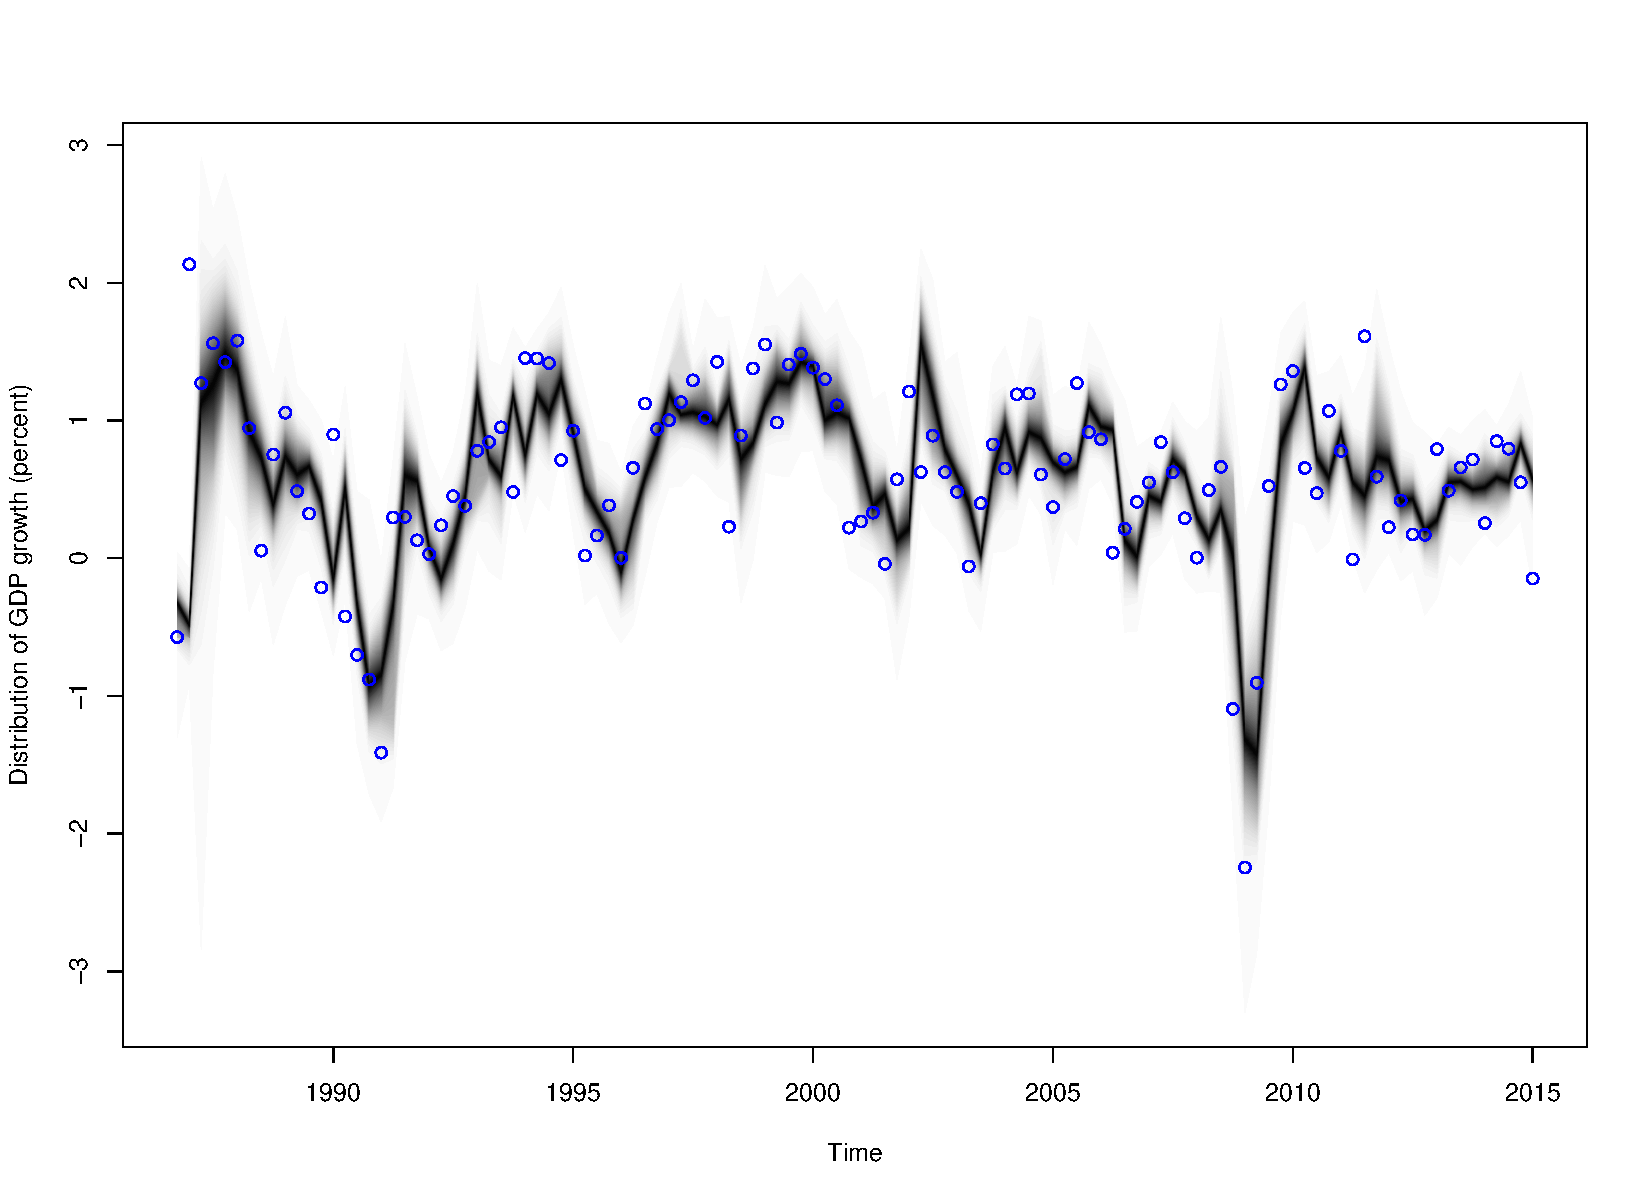
\includegraphics[width=0.6\linewidth]{Figures/forecast_distribution}
	\caption{Distribution of one step ahead forecasts for the observations}
	\label{fig:forecast_distribution}
\end{figure}



Figure  ~\ref{fig:forecast_distribution} shows the distribution of the one step ahead forecasts for the observations. The distribution of the one step ahead forecast for period $t$ is  made by using the value of GDP growth at $t-1$ and the observed covariates in regression component at time $t$. In Figure~\ref{fig:forecast_distribution}, the blue circle dots are observed GDP growth rate. The median of the distribution of forecast is colored black. To show the distribution, each 1\% quantile away from the median is shaded slightly lighter, until the 99th and 1st percentiles are shaded white. Figure  ~\ref{fig:forecast_distribution} shows the distribution of forecast is close to the observation except in some peculiar period such as the 2007 -2008 financial crisis period.




When we get the observation of GDP growth rate at time $t$, we can update the \textit{posterior} states at time t; 
$$ \alpha_t|GDP^t \sim N(m_t, C_t) $$ 
where $m_t =  a_t + R_t  f_t^\prime Q_t^{-1} (y_t - f_t)$, $y_t - f_t$ is the forecast error, and $C_t = R_t - R_t F_t^\prime Q_t^{-1} F_t R_t$ \cite{Petris2008}.


Figure  ~\ref{fig:states_distribution} shows that the posterior distribution of the state of the target variable GDP growth rate has much less variance than one step ahead forecast after the correction of forecast error. This is because that after we get the information of current observation for target variable, the state estimation is corrected through a weighting scheme.  The weight of the correction term is given by the gain matrix $K_t = R_t  f_t^\prime Q_t^{-1}$. A close look at Figure  ~\ref{fig:states_distribution} shows that after the correction, the posterior distribution of  the state is much closer to the observation than the one step ahead forecast.   


\begin{figure}[ht]
	\centering
	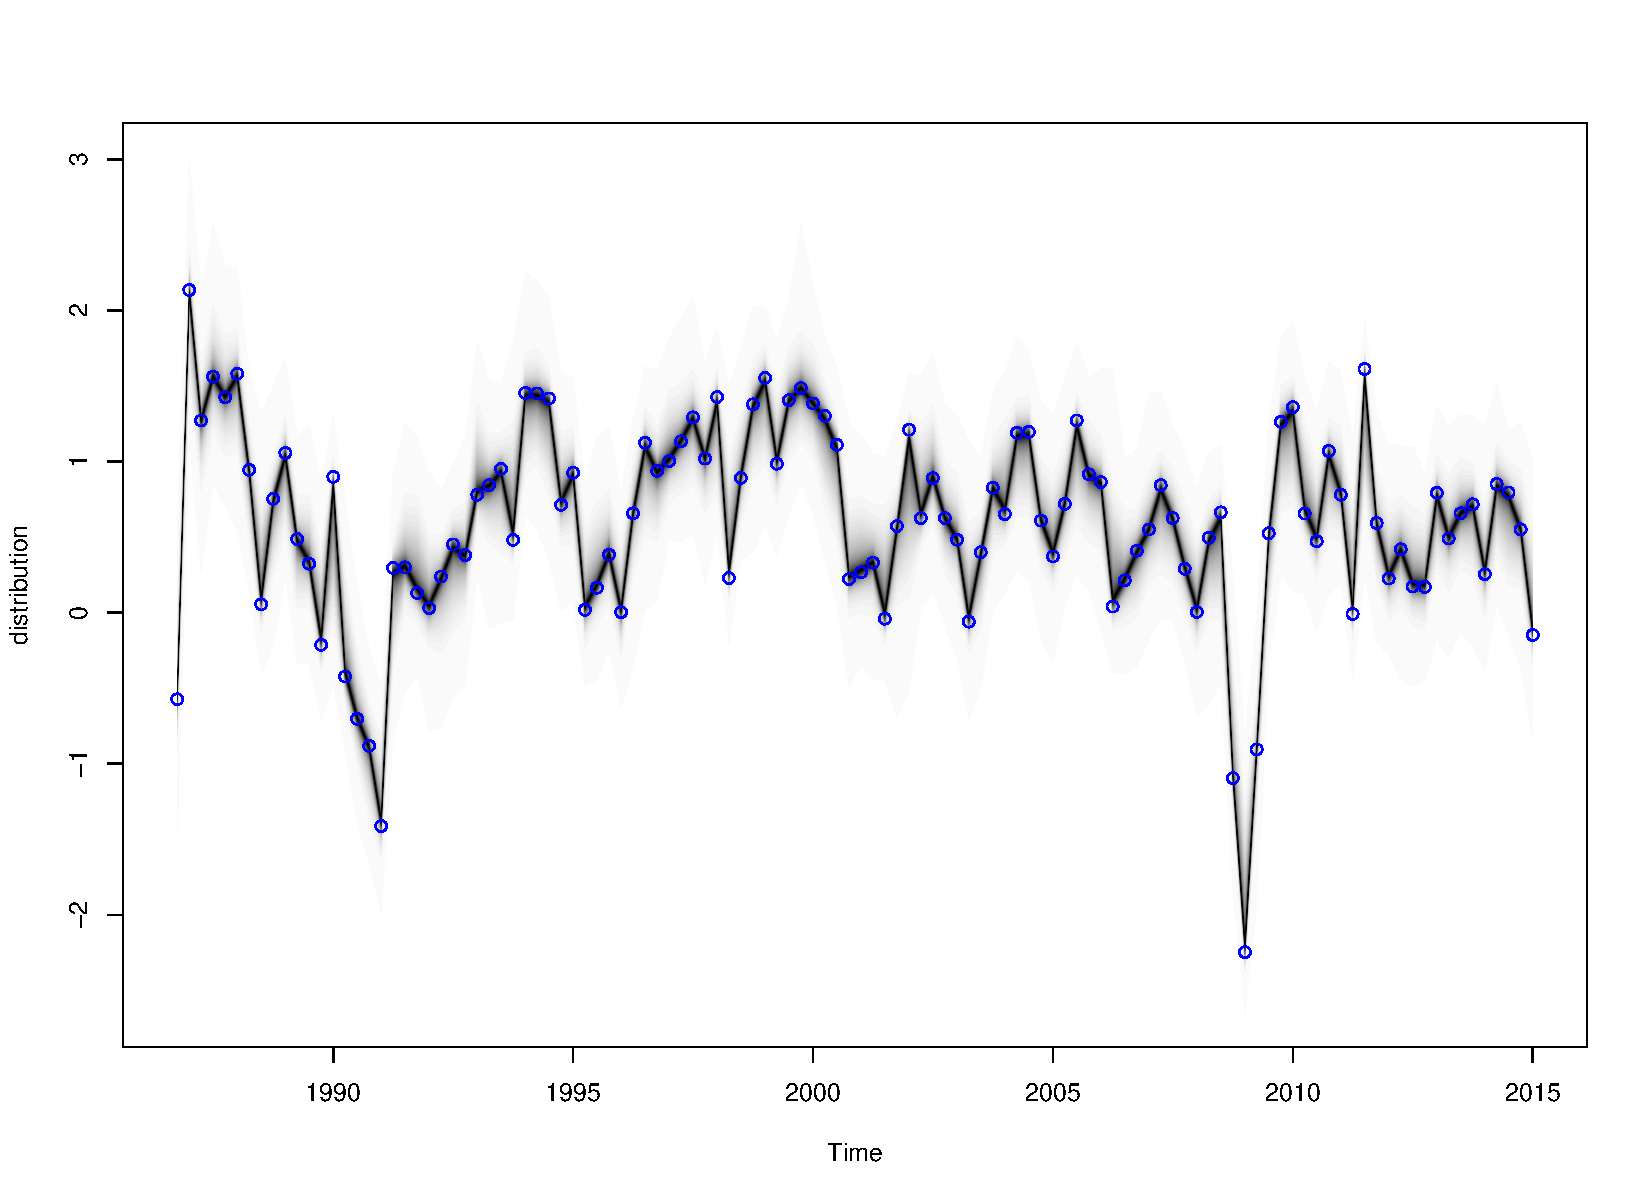
\includegraphics[width=0.6\linewidth]{Figures/states_distribution}
	\caption{Posterior distribution of states}
	\label{fig:states_distribution}
\end{figure}



\subsection{Diagnostic testing of  the model}

The difference also shows between the residual and forecast error. The residual is the difference between the posterior state and observation, and the forecast error is the difference between the one step ahead forecast and observation. 


\begin{figure}[ht]
	\centering
	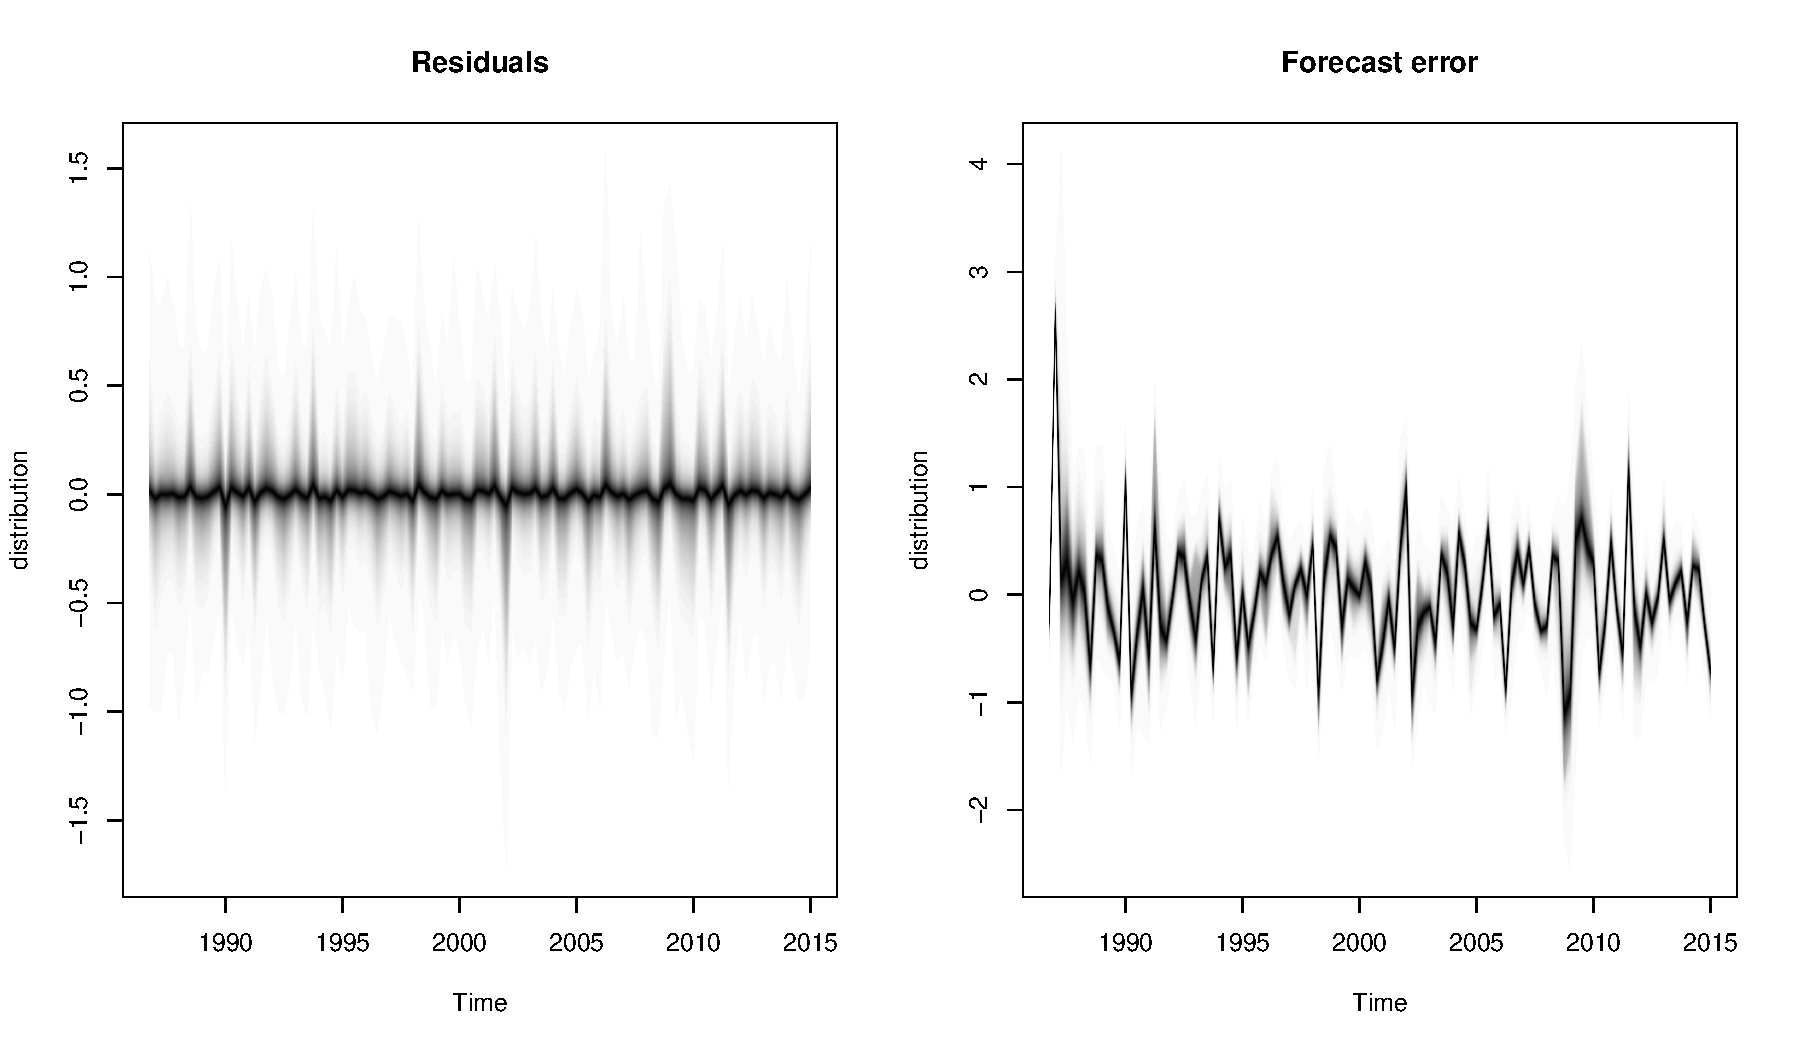
\includegraphics[width=0.8\linewidth]{Figures/residuals_prediction_errors}
	\caption{The distribution of the residual and forecast error}
	\label{fig:residuals_prediction_errors}
\end{figure}

In BSTS model, we assume the irregular error $\epsilon$ follows normal distribution. Figure  ~\ref{fig:residuals_prediction_errors} shows that the variation of the forecast errors is wider than the variation of the residuals. Both are centered at zero.  

\begin{figure}[ht]
	\centering
	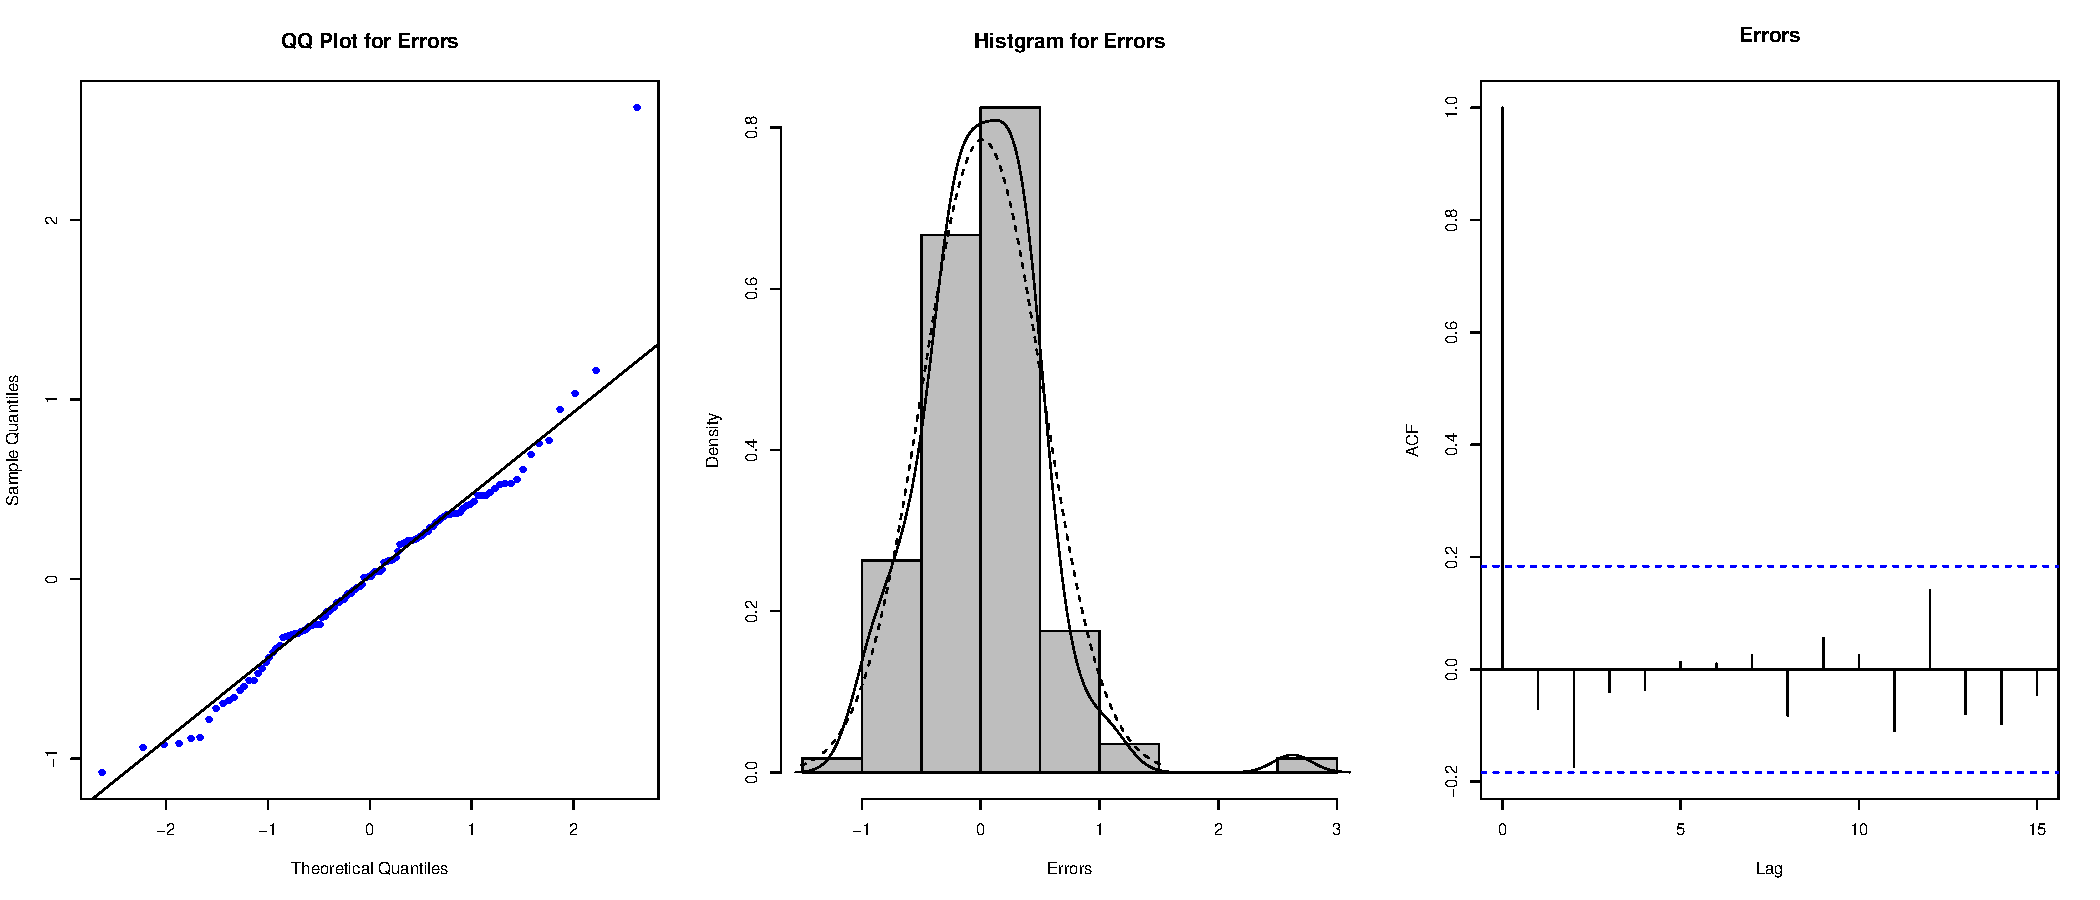
\includegraphics[width=1\linewidth]{Figures/errors3_hist}
	\caption{QQ plot, histogram, and ACF for one step ahead forecast errors}
	\label{fig:errors_hist}
\end{figure}


Figure  ~\ref{fig:errors_hist} shows that the distribution of one step ahead forecast errors is very close to normal distribution; however, it does not pass the  Shapiro-Wilk normality test. The forecast errors do  pass the Box-Ljung test, and do not show strong autocorrelation, which also can be verified by the ACF diagram in Figure  ~\ref{fig:errors_hist}. Of course, it is not necessary that forecast errors follow certain normal distributions, and we report these attributes of forecast errors just to illustrate the difference between forecast errors and residuals. In a state-space representation, the forecast errors and residuals are separately calculated in observation equation and state equation.      


\begin{figure}[ht]
	\centering
	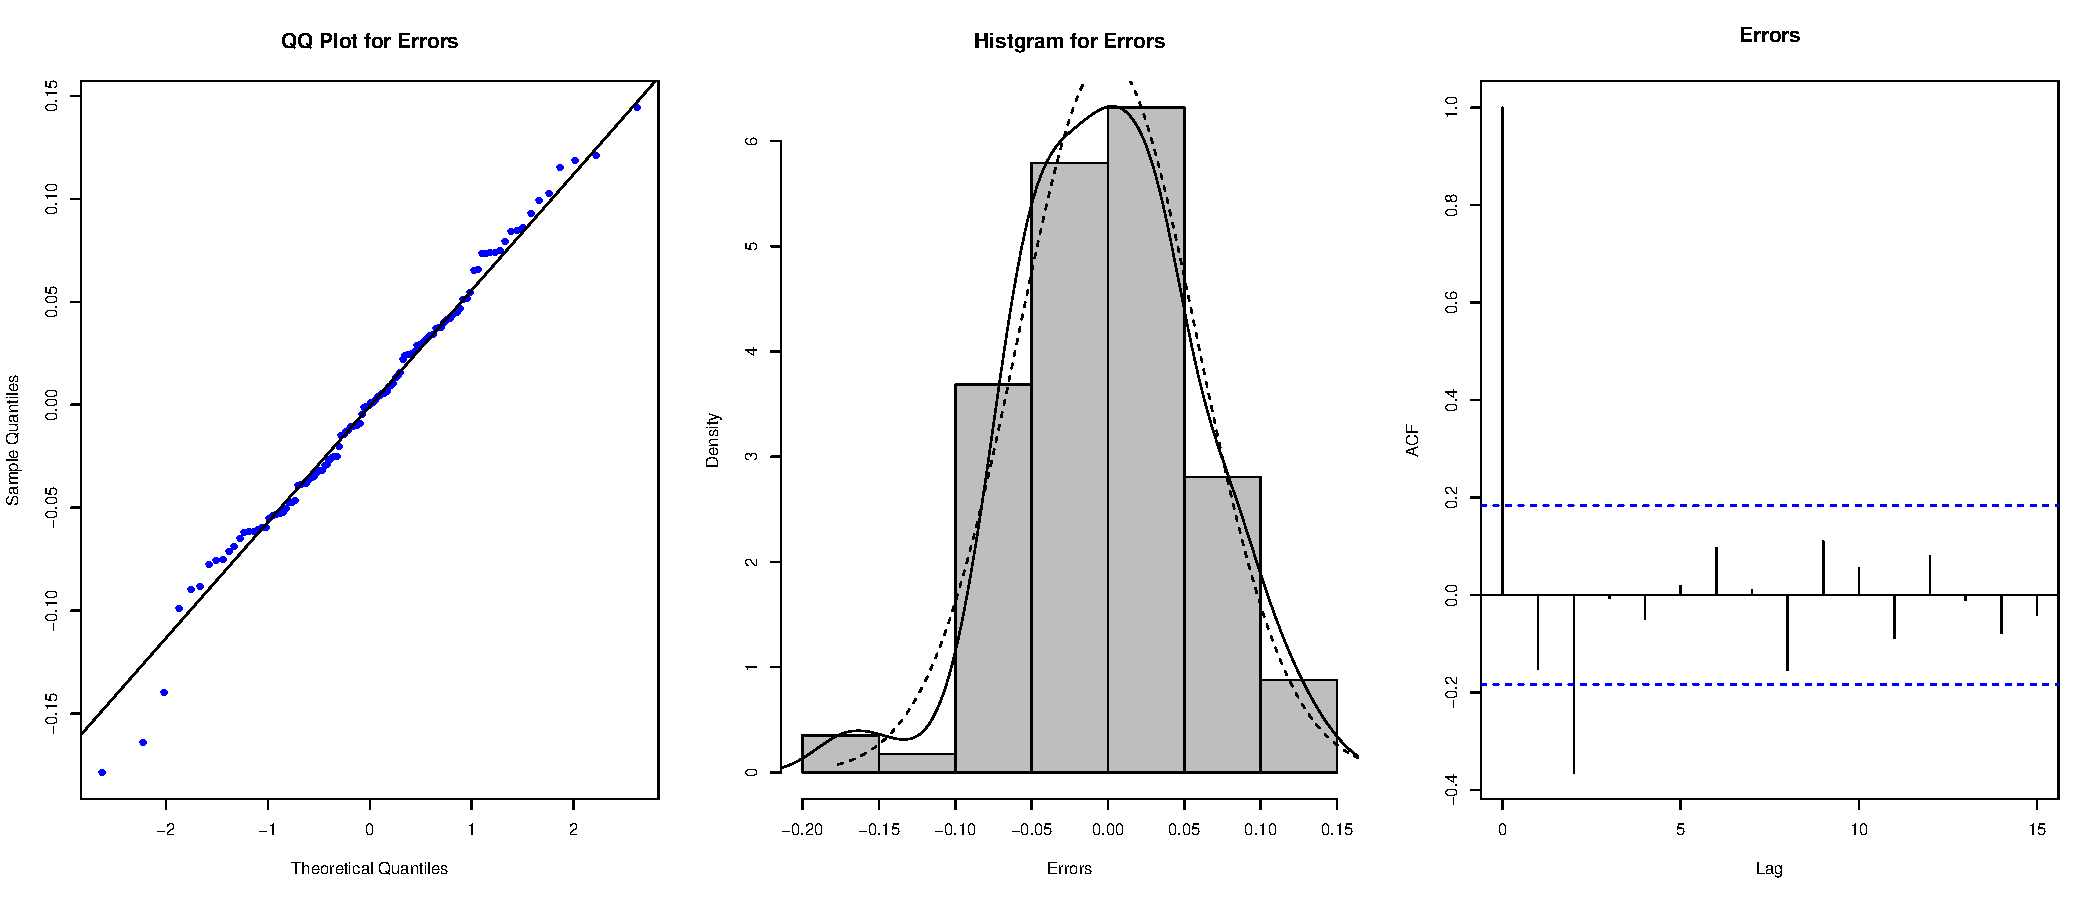
\includegraphics[width=1\linewidth]{Figures/residuals_hist}
	\caption{QQ plot, histogram, and ACF for residuals}
	\label{fig:residuals_hist}
\end{figure}


Figure  ~\ref{fig:residuals_hist} shows that the distribution of residuals is almost normal, and it does pass Shapiro-Wilk normality test. The residuals do not pass the Box-Ljung test, and show some evidences of autocorrelation, which also can be verified by the ACF diagram in Figure  ~\ref{fig:residuals_hist}. 

We also plot the trace plot for forecasts in the MCMC iterations. Most plot are stable after 2000 iteration, so we choose 2000 as brun-in parameter. 


\subsection{Contributions of components for GDP growth}

In our model, trend, AR terms and regression are three components besides the irregular error term. 
Figure  ~\ref{fig:components} shows how much variation in GDP growth can be explained by the trend and regression components. In Figure  ~\ref{fig:components}, the AR term is relatively stable, and the trend component is more volatile. The regression component exhibits more variation than the trend, which can help to capture the structural break or turning points in the  dynamics of the GDP growth. 


\begin{figure}[ht]
	\centering
	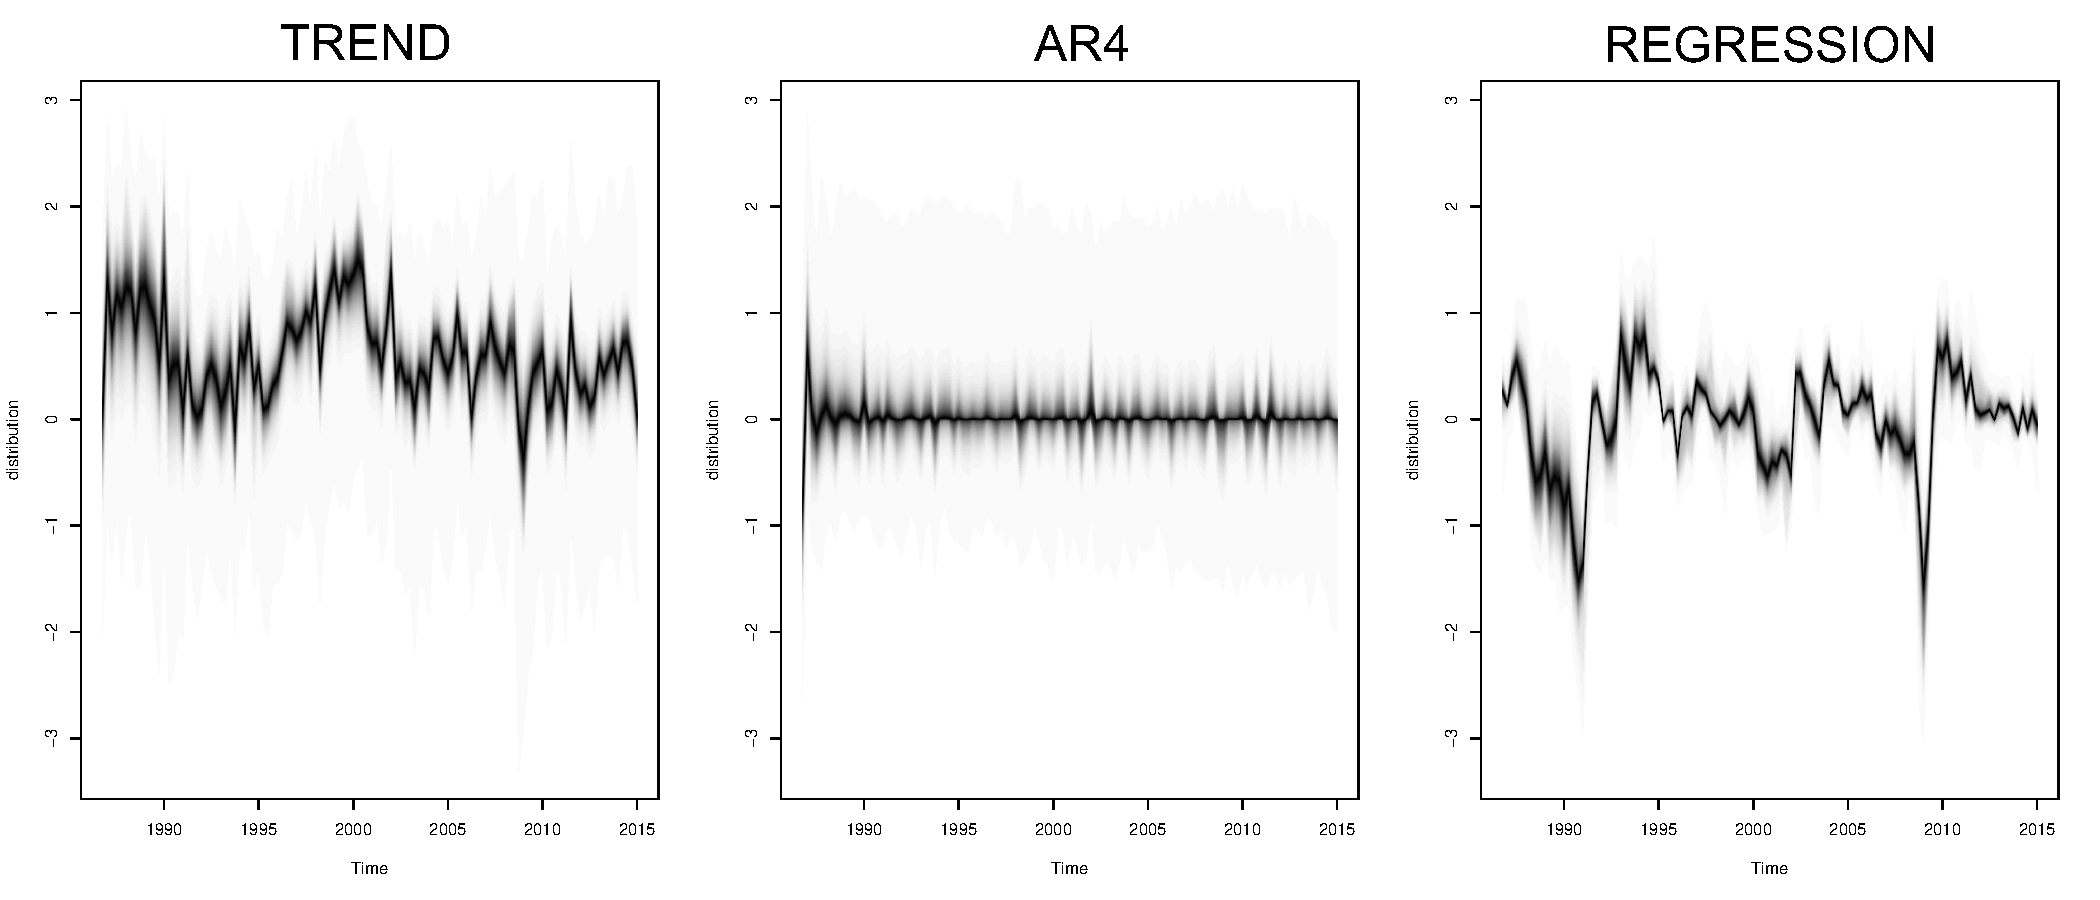
\includegraphics[width=1\linewidth]{Figures/components}
	\caption{Contributions to state for GDP growth}
	\label{fig:components}
\end{figure}




\subsection{The cumulative one step ahead forecast error for two models}

In order to illustrate the value of leading macroeconomic predictors, we fit a generalized local trend and AR(4) model without regression component and compare it with our model 3.  The cumulative sum of the absolute values of the one step ahead forecast errors for the two models is shown in Figure ~\ref{fig:cumulative_errors}. The bottom part of Figure ~\ref{fig:cumulative_errors} shows the scaled value of the target variable GPD growth. The model 3 performs better, especially during the 2008 to 2009 financial crisis, which emphasizes one of the advantages of BSTS-U-MIDAS: it is robust to change points and structural break.


\begin{figure}[ht]
	\centering
	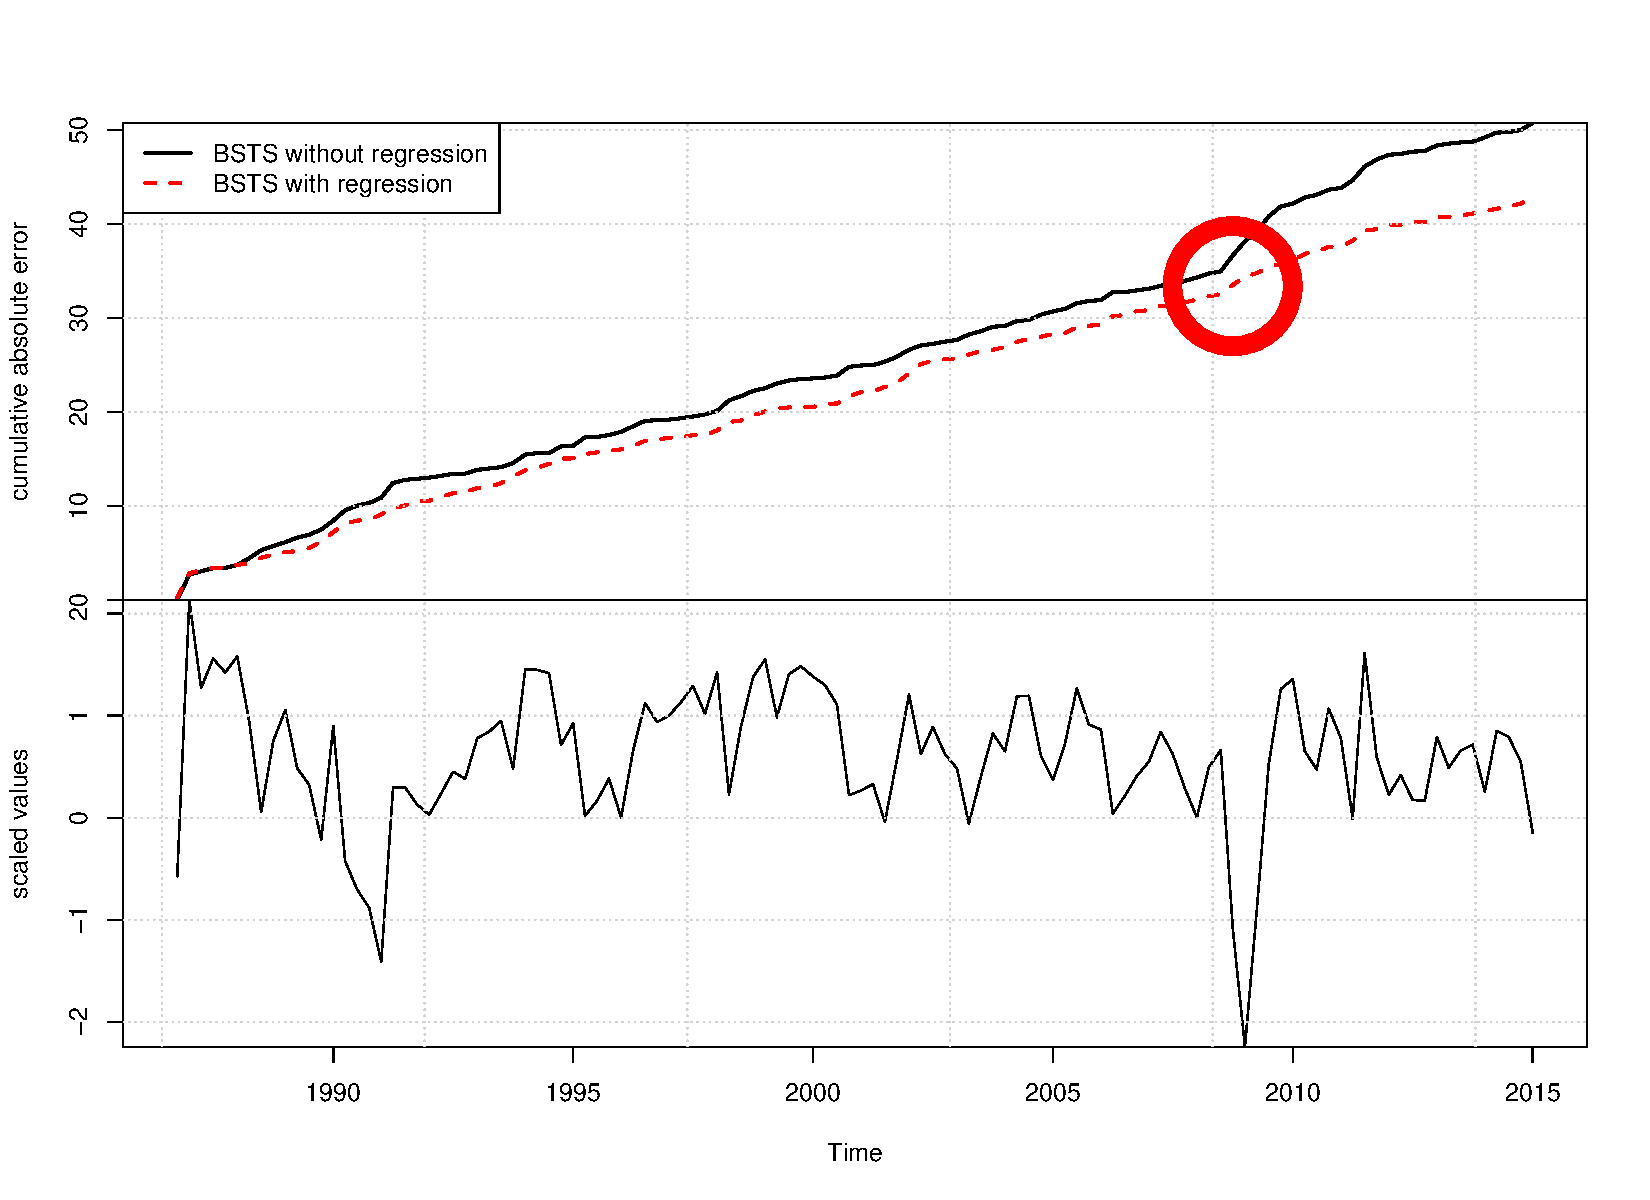
\includegraphics[width=0.6\linewidth]{Figures/cumulative_errors}
	\caption{The cumulative absolute one step ahead forecast error}
	\label{fig:cumulative_errors}
\end{figure}


The cumulative sum of the forecast errors for model without regression component jumps when the recession starts at 2008. However, the cumulative sum of the forecast errors for model 3 increases at a constant rate. In BSTS with regression model, the signal among those leading predictors helps to capture the economic forces which drive the dramatic change in the target variable.  

The robustness to structural break of the BSTS-U-MIDAS could be very helpful for us to predict recessions or boom periods. 

\subsection{The predictors with high inclusion probability}

Another thing of interest in our forecast  is to find out which predictor is significant according to its ability for helping predict the variation of GDP growth in Canada.


\begin{figure}[ht]
	\centering
	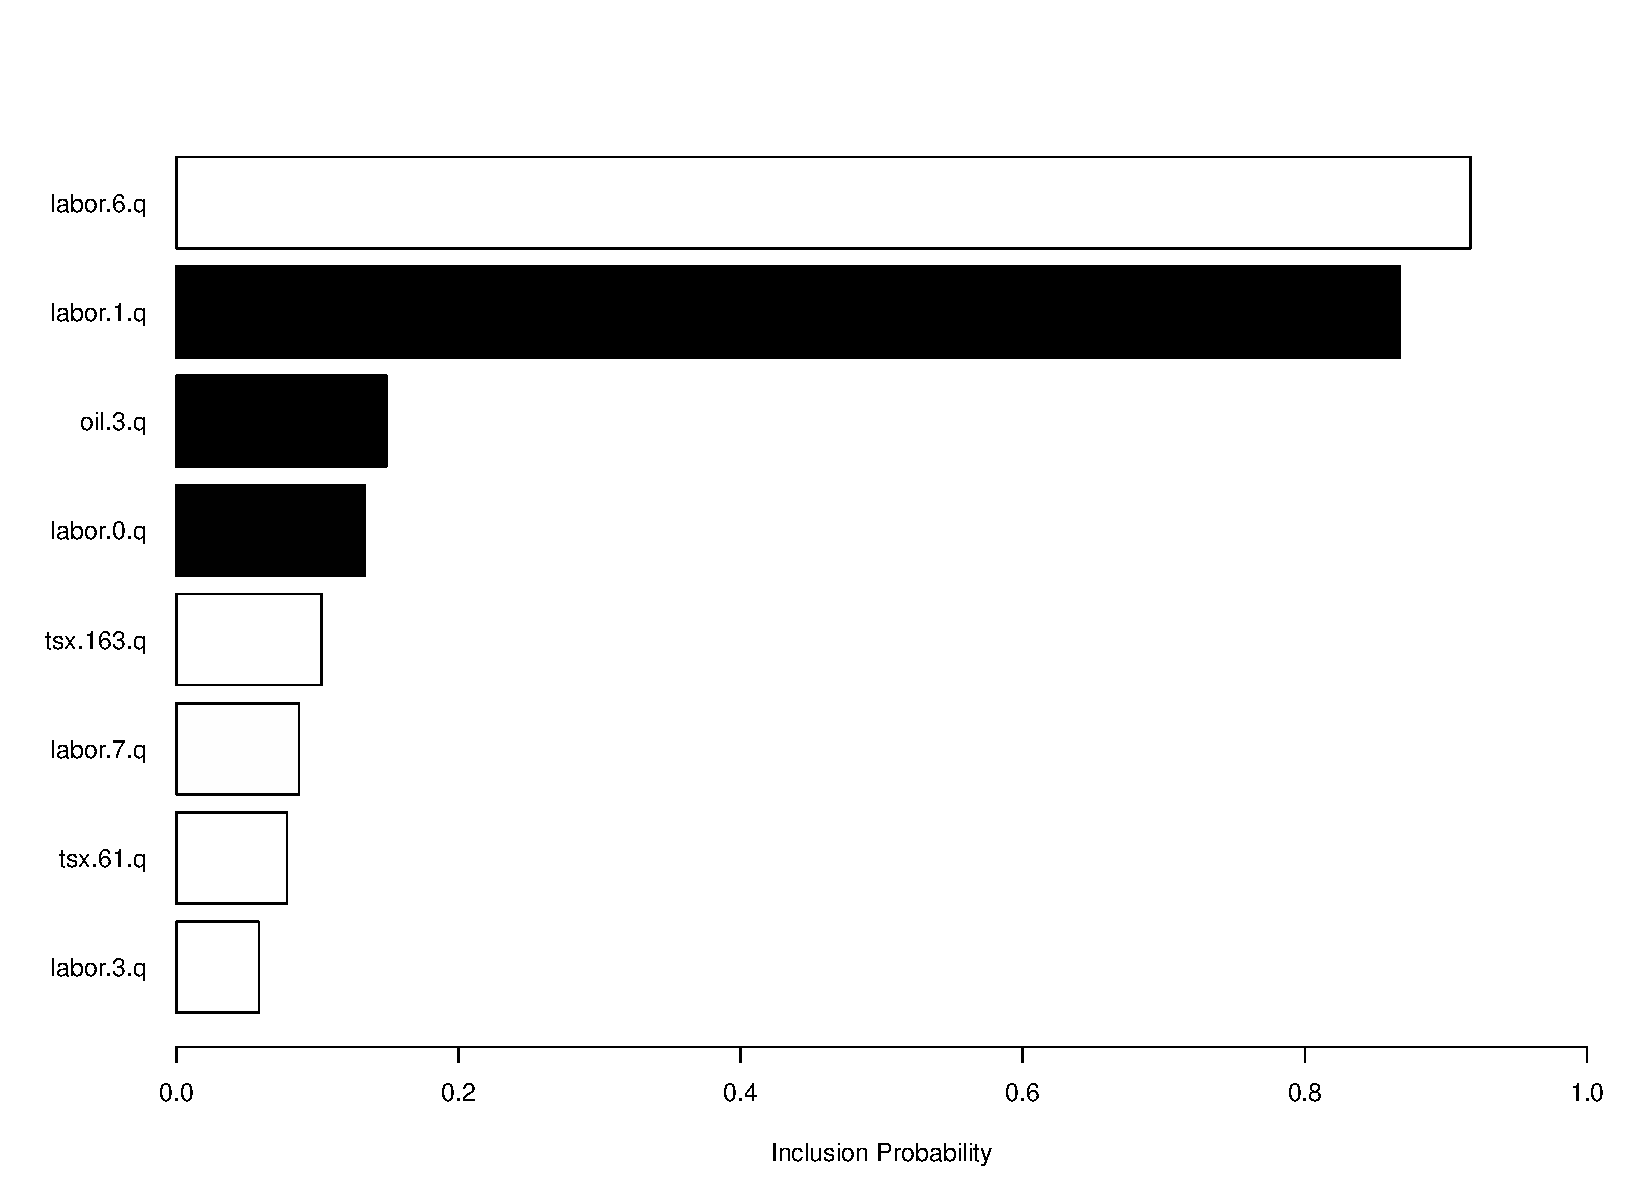
\includegraphics[width=0.6\linewidth]{Figures/Coefficients}
	\caption{Predictors with inclusion probability greater than 5\%}
	\label{fig:Coefficients}
\end{figure}


Figure ~\ref{fig:Coefficients} shows the predictors with inclusion probability in MCMC iterations greater than five percent. A white bar indicates that the predictor has a positive relationship with target variable, and a black bar indicates a negative relationship. The size of the bar represents the inclusion probability. 



The unemployment rate is labeled as ``labor", TSX stock market index return is labeled as ``tsx", and oil price return is labeled as ``oil". The ``labor.0.q" represent the most recent observation for the unemployment rate. In our model, ``labor.0.q" is the unemployment rate for the last month in the reference quarter. ``labor.6.q" is fourth month before the reference quarter.For example, the last target quarter is first quarter 2015, and then the last ``labor.0.q" observation is the  unemployment rate for March 2015. The last ``labor.6.q" value is the unemployment rate for September 2014. 

Likewise, for daily data, ``oil.3.q" is oil price return (log difference of oil price) in May 25, 2015, three days before May 28, 2015. ``tsx.61.q" is stock market return sixty one business days before May 28, 2015, one day in March 2015.  The locations of predictors with high probability on time table  are illustrated in Figure ~\ref{fig:MonthQuarterYear}. The background color shows the availability of the data. A white background represents the observation in that period is not available, and a yellow background shows that observation is available. 


The ragged yellow cells demonstrate the different publication lags for those variables. Since the publication lag for GDP in Canada is about two months, we get chance to utilize the heading high frequency data extending to two monthes. For example, Statistics Canada released first quarter's GDP on May 30, so we can practice forecasting for first quarter's GDP till May 29. That is why the daily data are available on time table till the end of May. In this sense, our practice can be called now-cast since we forecast a figure which is already there but has not been observed by using more recent high frequency data.  


The boldface number in green cell means the lagged numbers of predictors and this predictor has a positive relationship with GDP growth. The italicized and underlined number in shaded cell means the lagged numbers and this predictor has a negative relationship with GDP growth. For example, the ``labor.0" and ``labor.1" have a negative relation with GDP growth.




\begin{figure}[ht]
	\centering
	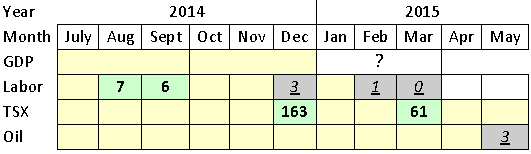
\includegraphics[width=1\linewidth]{Figures/MonthQuarterYear}
	\caption{Predictors with high inclusion probability on time table}
	\label{fig:MonthQuarterYear}
\end{figure}


The signs of the coefficients of the predictors mostly meet our anticipation based on economic theory. For example, the stock market return is positively related to GDP growth. However, some others do not. For example, the top predictor ``labor.6.q" is positively related to GDP growth. If we take the MIDAS into account, and we will anticipate a certain combination of high frequency data should work as a predictor for a low frequency counter part. As we see in Figure ~\ref{fig:Coefficients} and Figure ~\ref{fig:MonthQuarterYear}, the ``labor.0" and ``labor.1" in March and February 2015 combined with ``labor.6" and ``labor.7" in September and August 2014 help us predict GDP growth. Specifically, the scenario, that  unemployment rates were low two quarters ago and high in this quarter, means the GDP growth in this quarter is going to be low. 
It turns out that one single high frequency time series is not sufficient for forecasting. Only the combination of several time series works. This phenomenon also shows in Figure ~\ref{fig:GDPincremental}. 


\begin{figure}[p]
	\centering
	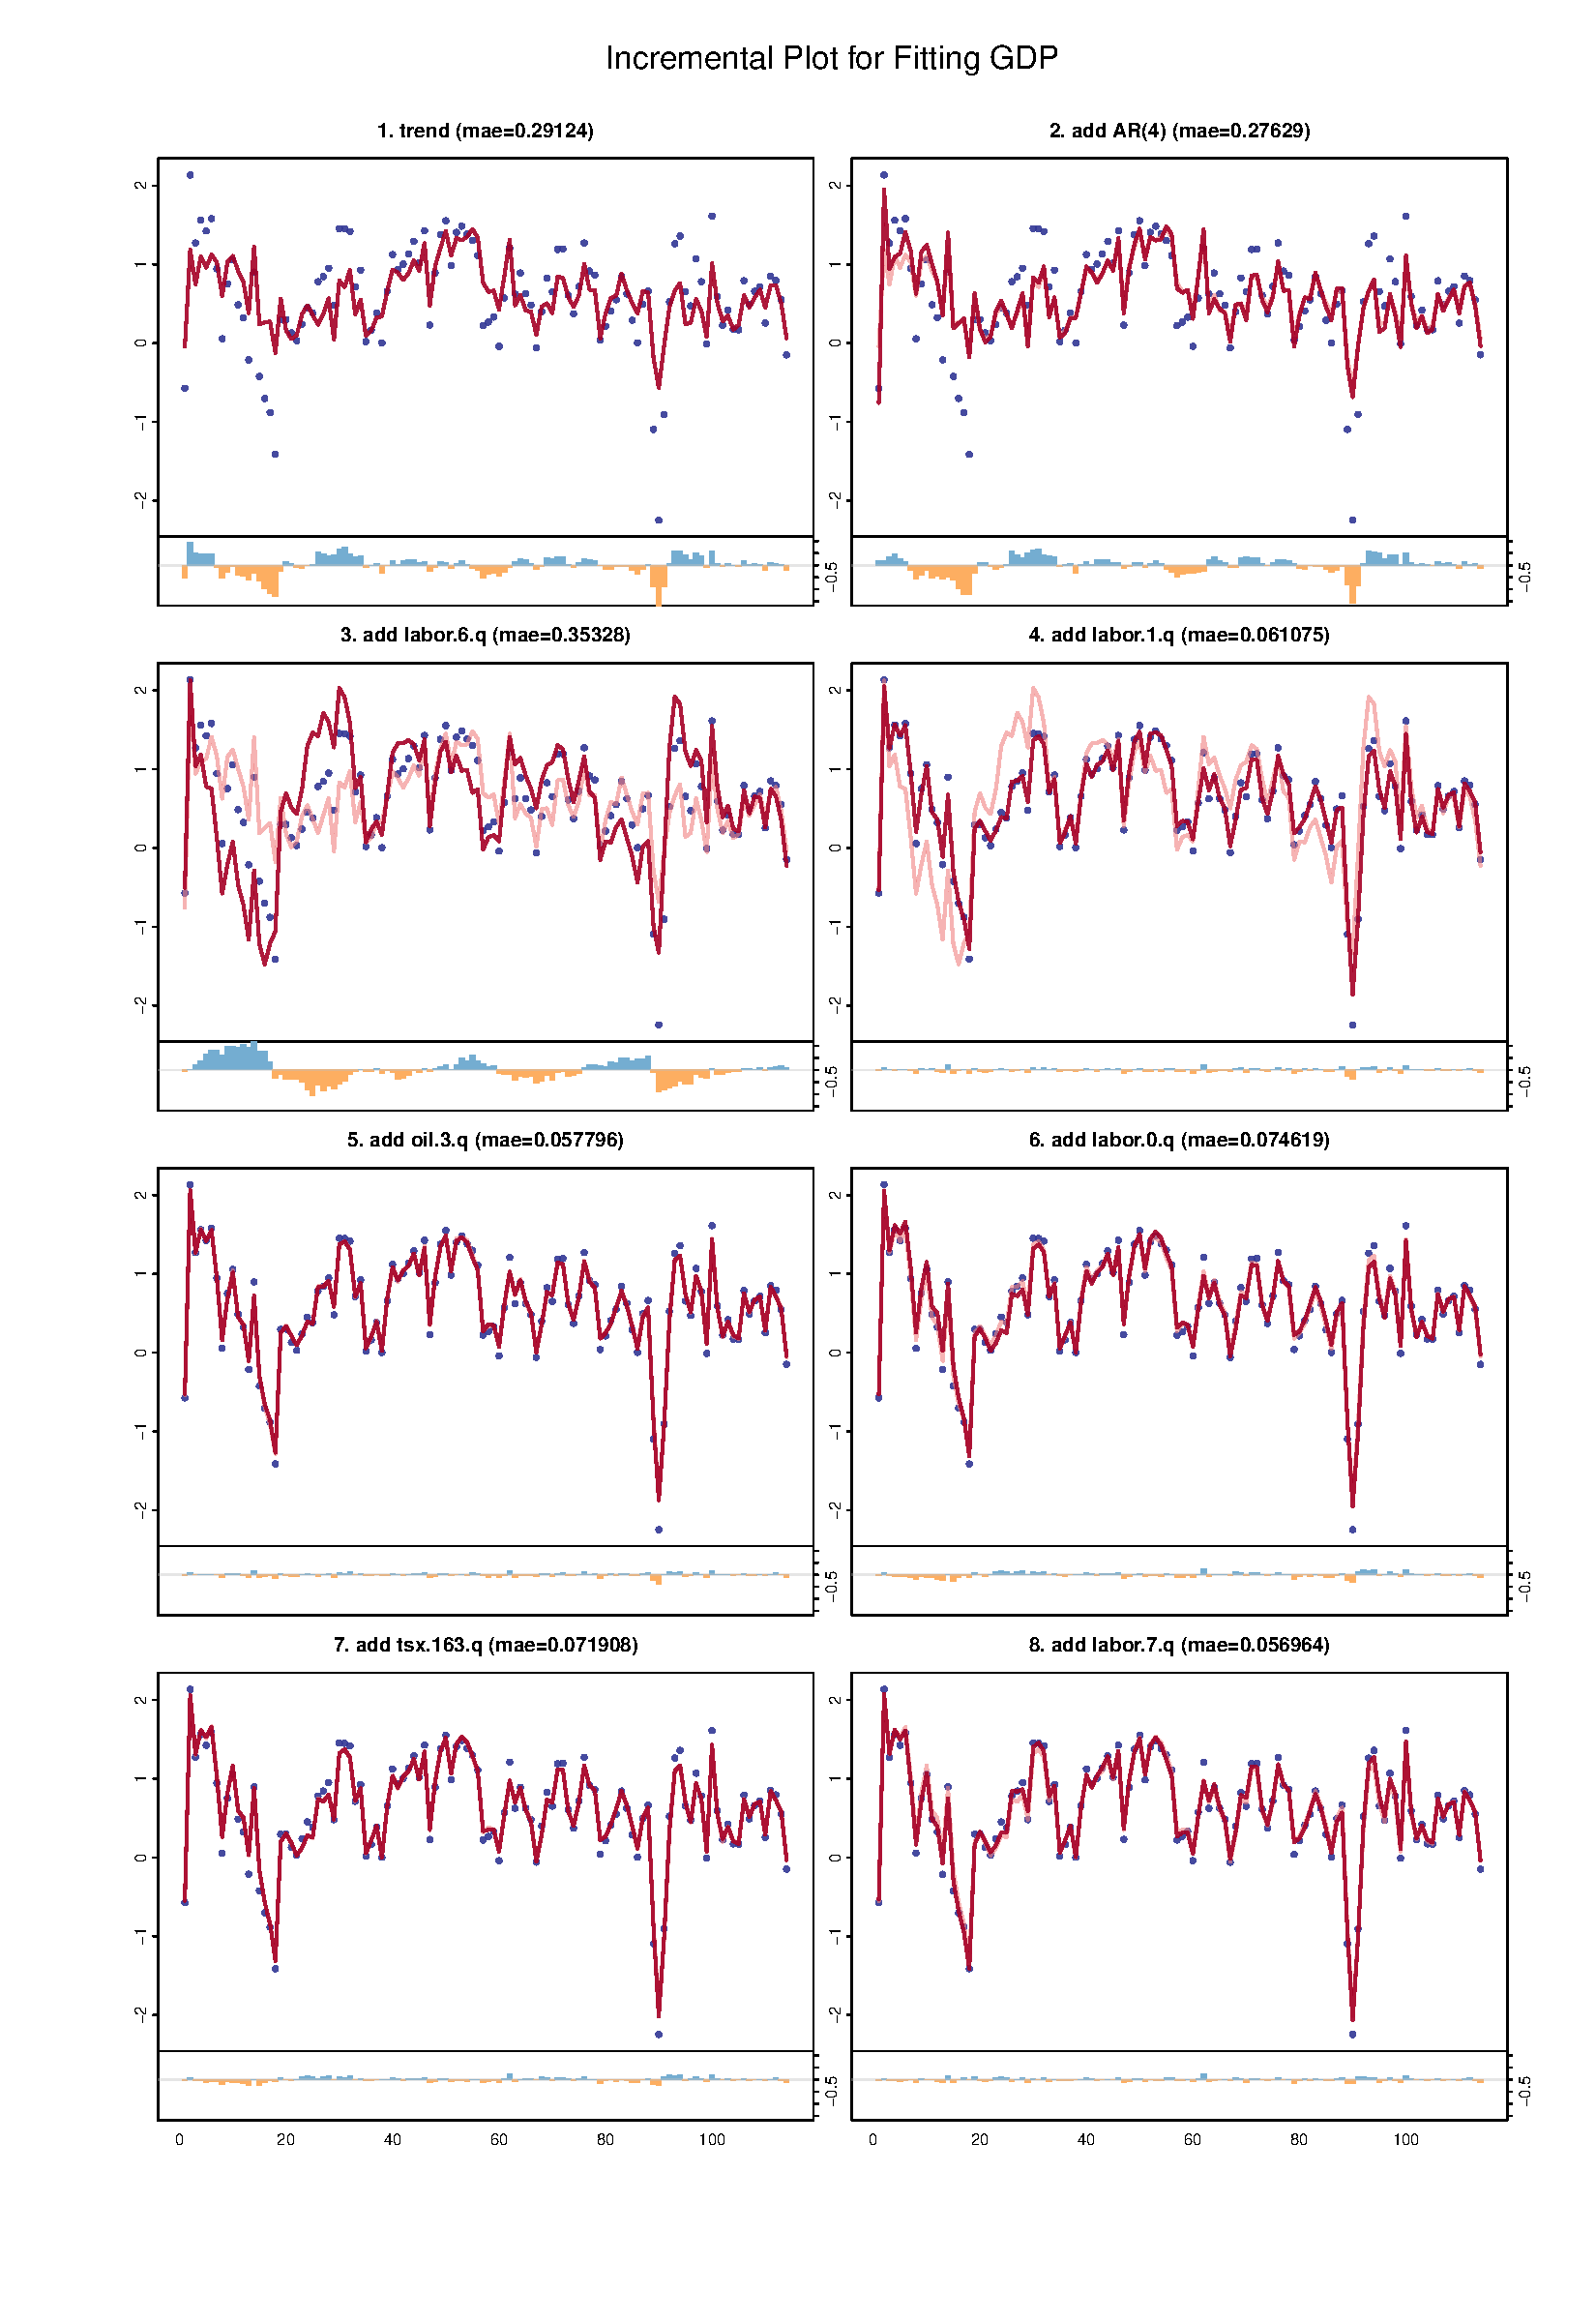
\includegraphics[width=0.8\linewidth]{Figures/GDPincremental}
	\caption{Decomposition of forecast for GDP growth}
	\label{fig:GDPincremental}
\end{figure}

Figure ~\ref{fig:GDPincremental} shows the contribution of each state component and predictor to the fit of model. Variables are ordered by probability of inclusion. The mean absolute error in terms of the posterior distribution of the state of GDP growth is given in the title. The faint line in each panel is the previous fit, and the residuals are shown at the bottom of each panel. 

It is interesting that after including ``labor.6" in model, the MAE and residual increase. The MAE and residuals continue decreasing  after  ``labor.1" included. This phenomenon shows that individually including one specific predictor may not improve forecasting, but jointly including a set of predictors might improve forecasting a lot. 


Another thing we can take away from Figure ~\ref{fig:Coefficients} is that BSTS-U-MIDAS gives us a sparse model. The top two predictors have over 80 percent inclusion probability in MCMC iterations. Others have less probability. This pattern also is  verified by the distribution of the size of model in Figure ~\ref{fig:size} 

\begin{figure}[h]
	\centering
	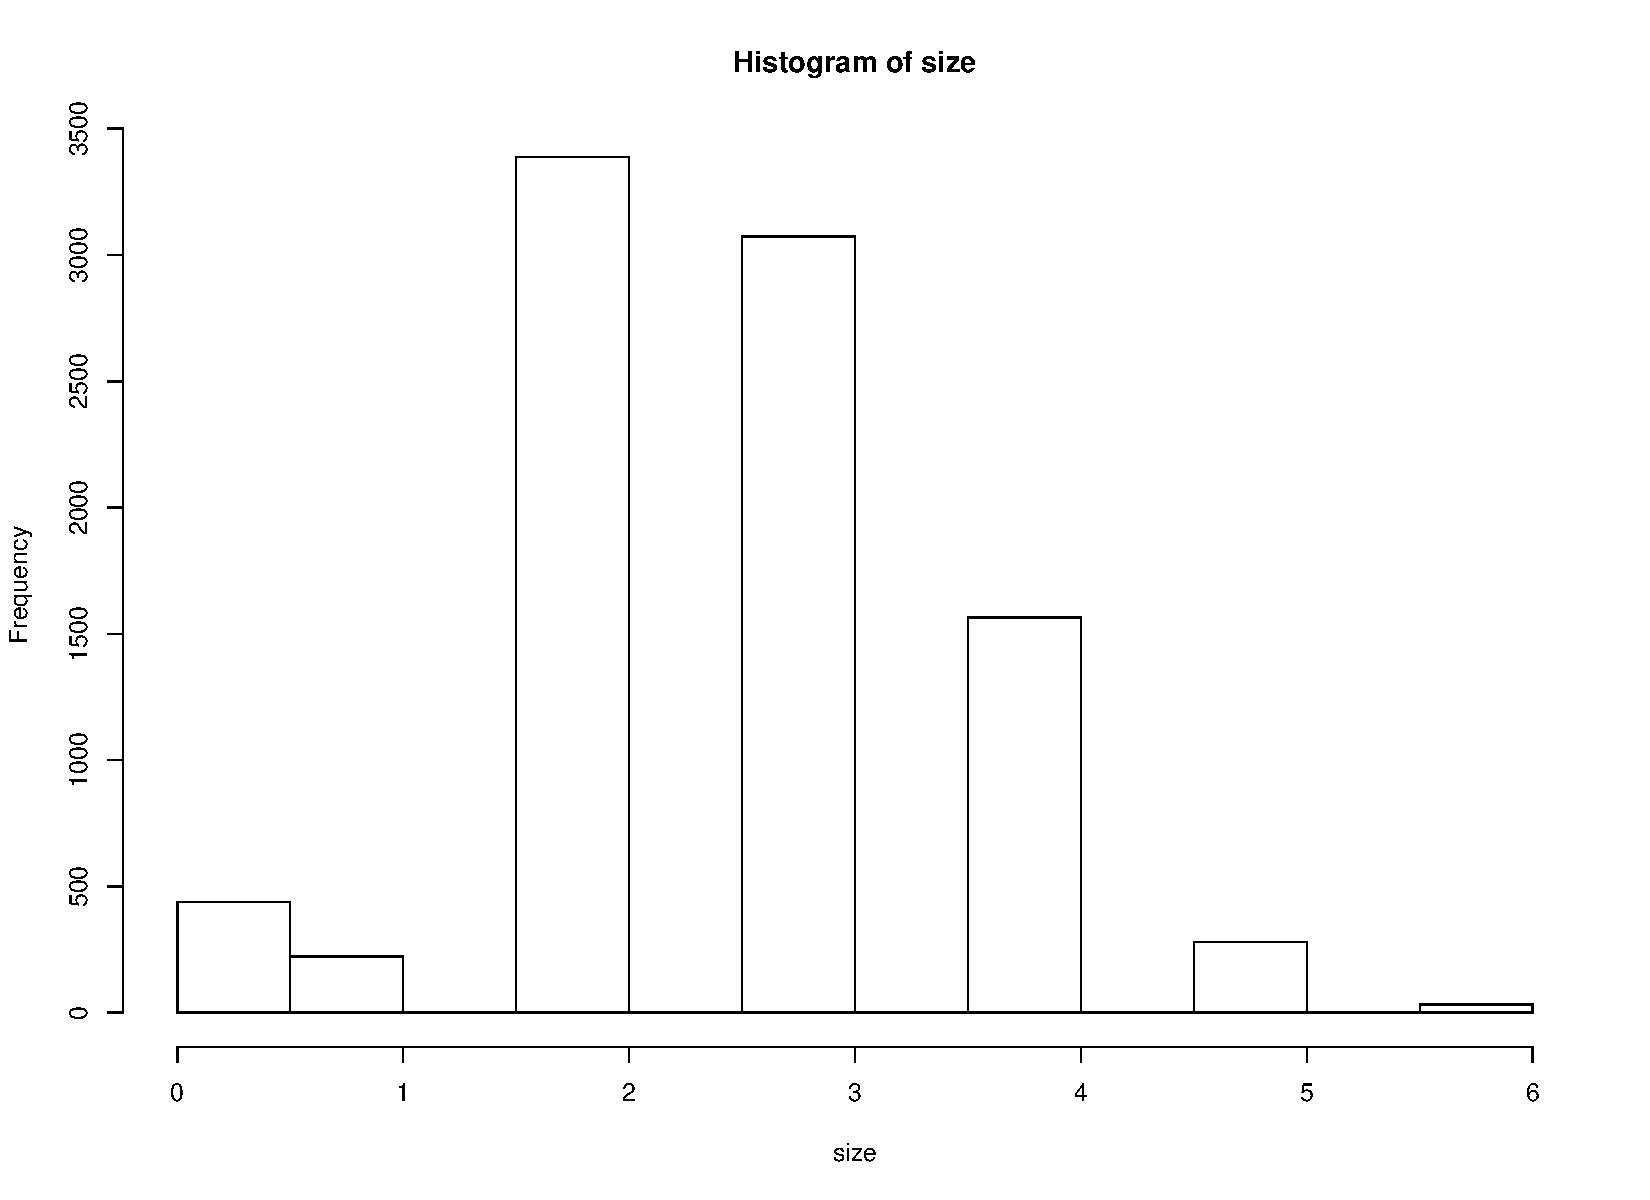
\includegraphics[width=0.5\linewidth]{Figures/size}
	\caption{The posterior distribution of  model size}
	\label{fig:size}
\end{figure}

Figure ~\ref{fig:size} shows the posterior distribution of the number of predictors in the model. We have 600 variables  to choose from in model 3. The median number of the distribution of model size in model 3 is 3. The largest model in the MCMC sample has 6 predictors. The BSTS-U-MIDAS model indeed gives us sparsity.  
 
In the top 100 predictors with high inclusion probability, there is no housing start data. One possible reason is that the housing data we have collected are not representative, so they are not included in many MCMC iterations. However, they are not absolutely excluded from the model. Some variables from ``house" family still have 0.01 percent inclusion probability. Through the Bayesian model averaging, the information in ``spread" and ``house" family still will be conveyed into the final model, so they still have impact on the final forecasts.


\begin{figure}[h]
\centering
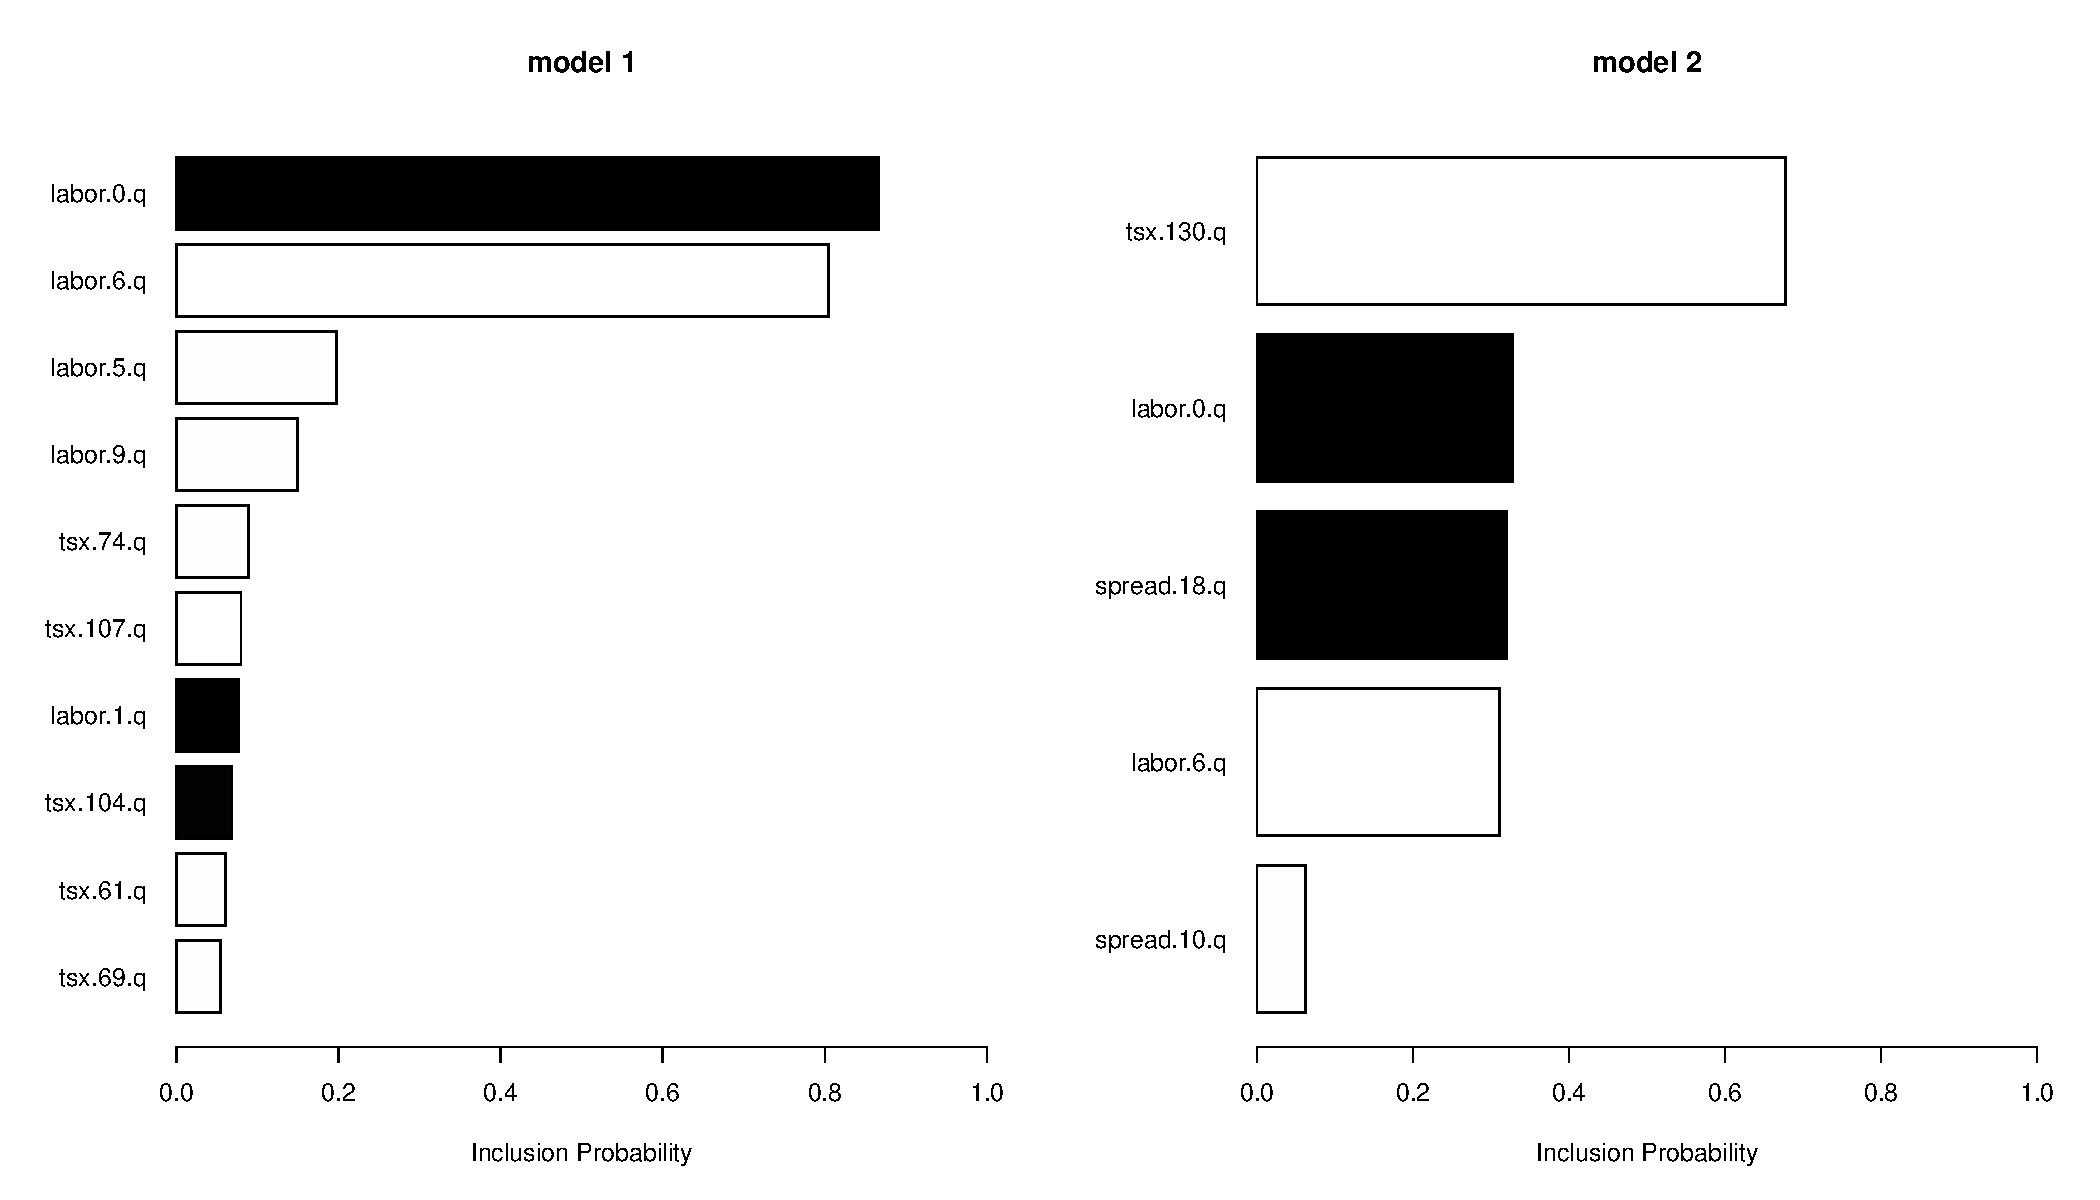
\includegraphics[width=0.7\linewidth]{Figures/Coefficients_model1_2}
\caption{Predictors with inclusion probability greater than 5\%}
\label{fig:Coefficients_model1_2}
\end{figure}


Figure ~\ref{fig:Coefficients_model1_2} shows the predictors with inclusion probability greater than 5\% in model 1 and model 2. The composition of top predictors changes after the housing starts data is included in model 2. Even the model size also changes, which is shown in Figure ~\ref{fig:size_1_2}.


\begin{figure}[ht]
\centering
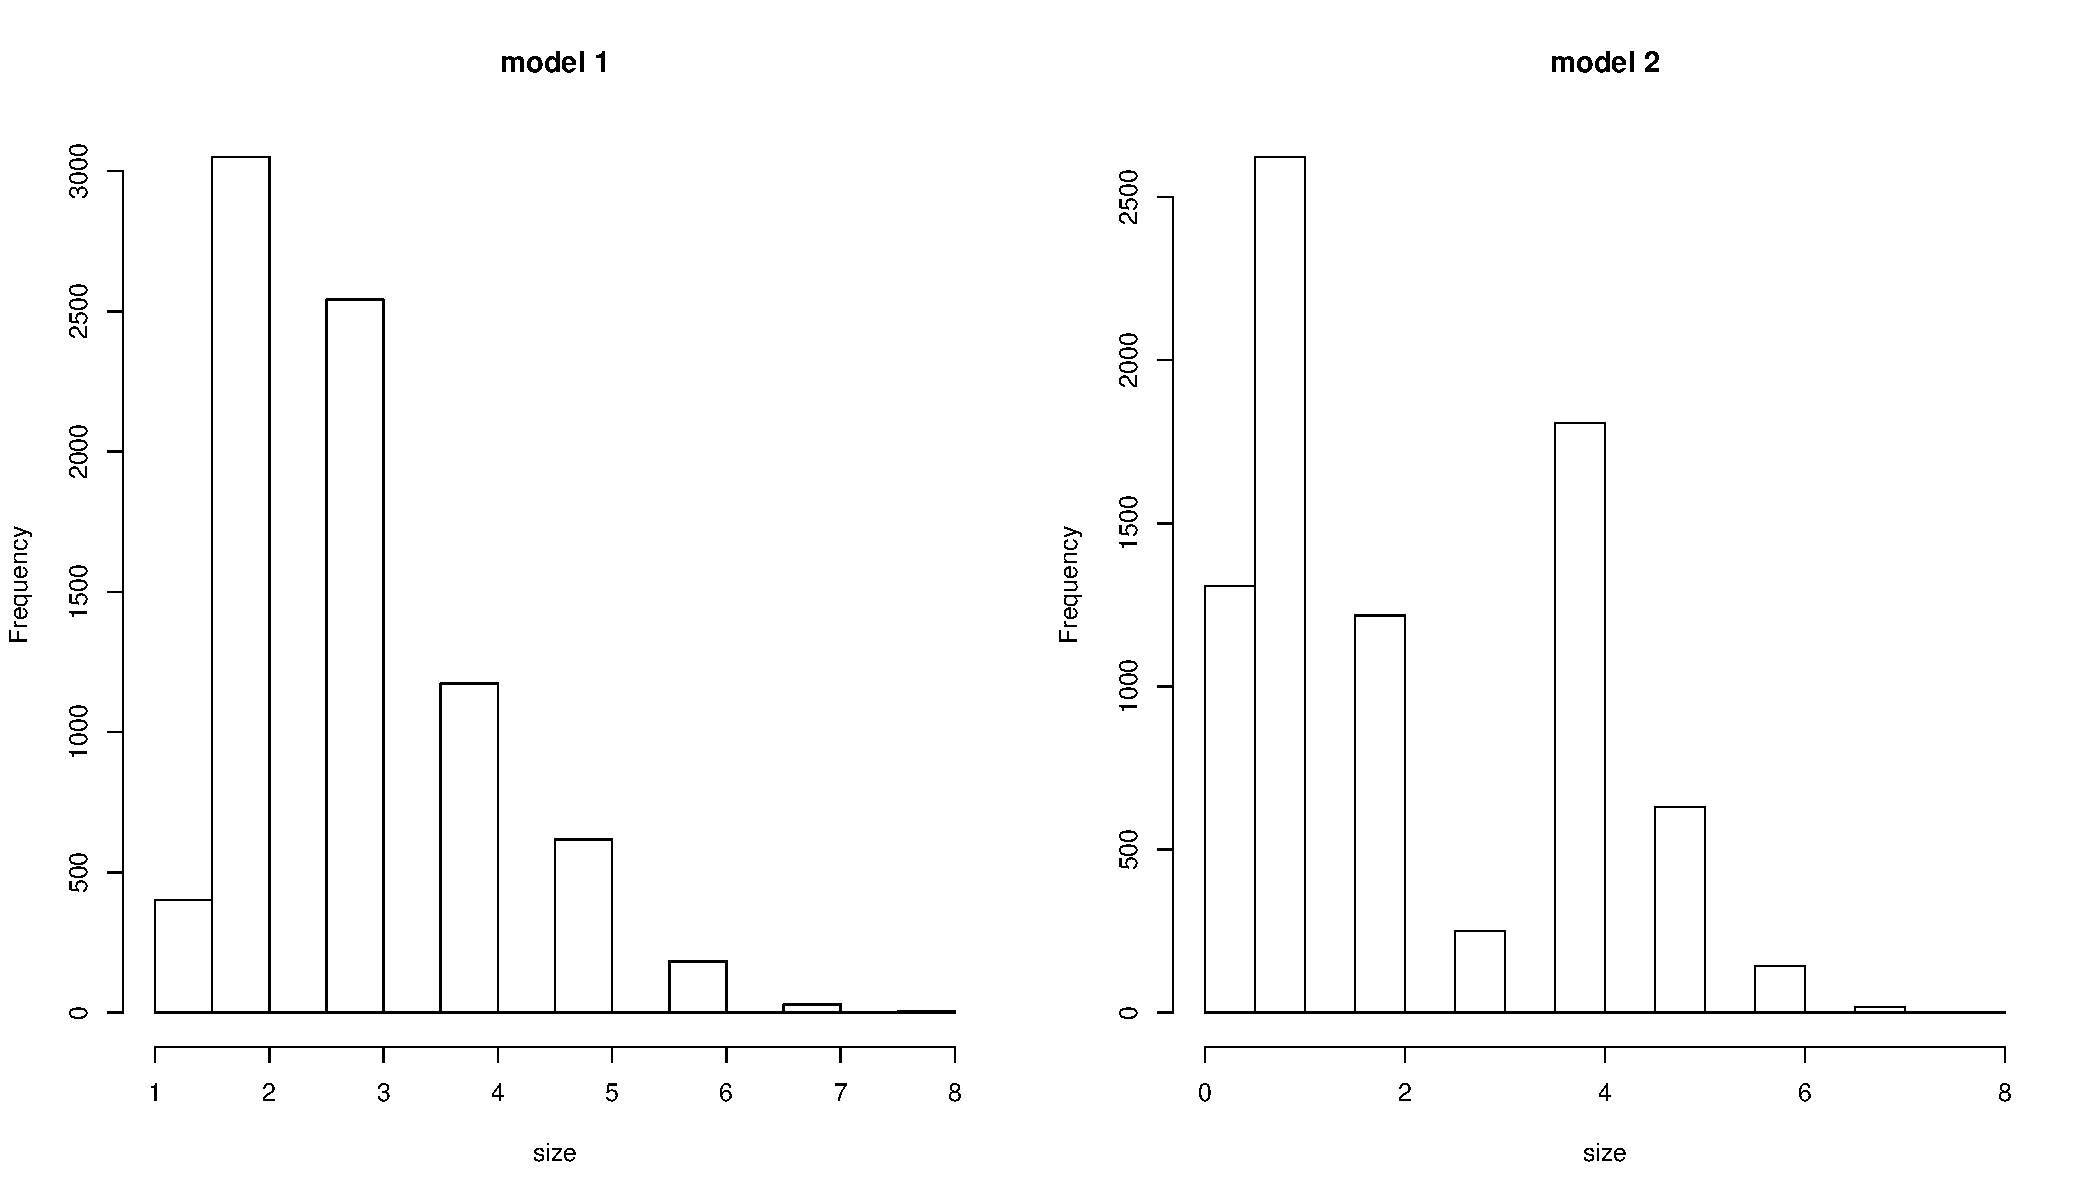
\includegraphics[width=0.6\linewidth]{Figures/size_1_2}
\caption{The distributions of the size of model 1 and model 2}
\label{fig:size_1_2}
\end{figure}
 
Suppose the housing data is noisy in some sense. After the housing data is included in the model, the inclusion probability of the top predictors decreases, and the size of the model decreases. Every single model in the MCMC iterations becomes more sparse and weaker in terms of forecast ability. It shows BSTS-U-MIDAS model can suffer from noisy or redundant data. However, when we include the oil return data into model 3, the performance of model 3 gets better, even better than model 1. The reason might be because when more relevant predictors are included in the model, the inclusion probability of less relevant predictors are pushed towards zero.   


% Please add the following required packages to your document preamble:
% \usepackage{booktabs}
\begin{table}[ht]
	\centering
	\begin{tabular}{@{}llllll@{}}
		\toprule
		          & ME     & RMSE     & MAE      & MPE      & MAPE     \\ \midrule
		Model 1    & -219.327 & 7548.331 & 6100.694 & -0.012 & 0.386 \\
		Model 2    & -256.496 & 8161.589 & 6625.706 & -0.013 & 0.419  \\ 
		Model 3    & -159.853 & 6952.102 & 5641.339 & -0.008 & 0.356\\ \bottomrule
	\end{tabular}
	\caption{Comparison of forecast error 2003-2015 in model 1, 2, and 3}
	\label{ErrorCom123}
\end{table}

We select second quarter in 2003  to first quarter  in 2015  as our forecast horizon. We compare the performance of three models in terms of GDP, which is shown in Table ~\ref{ErrorCom123}.  Model 2 with housing starts data  performs slightly worse than model 1. Model 3 with housing starts and oil return data performs best.

\section{Comparison Between BSTS, ARIMA, and Boosting Model}

We also compare one step ahead forecast performance between BSTS-U-MIDAS, ARIMA and Boosting models. ARIMA is a benchmark which is a normal practice in the  forecasting business. The Boosting model has many advantage similar to BSTS-U-MIDAS. It can deal with a large numbers of predictors and is robust to over-fitting. It ensembles many weak classifiers or regression trees to get a good prediction, which is similar to Bayesian model averaging in the BSTS-U-MIDAS model. Boosting model allows us to model complex relationships among the large data set by using more flexible model (non-linear) instead of simple linear models\cite{Varian}.  


The ARIMA model is implemented by automatic `arima' algorithm of the Forecast package in R \cite{Hyndman2008}. The Boosting model is implemented by the GBM package in R \cite{Ridgeway2015}. All forecast are one step ahead  forecasts which are estimated in a recursive way. We refit the model every time when the forecast horizon extends to the next period. (See appendix D for details.)

We take data from third quarter in 1980  to first quarter in 2003 as the training period and second quarter in 2003 to  first quarter in 2015 as the test period. We predict the GDP growth rate and the level of GDP for Canada from second quarter 2003 to  first quarter 2015. For visual comparison, we use GDP growth rate since the level of GDP changes a lot from the second quarter in 2003 to  first quarter in 2015. 


\begin{figure}[h]
	\centering
	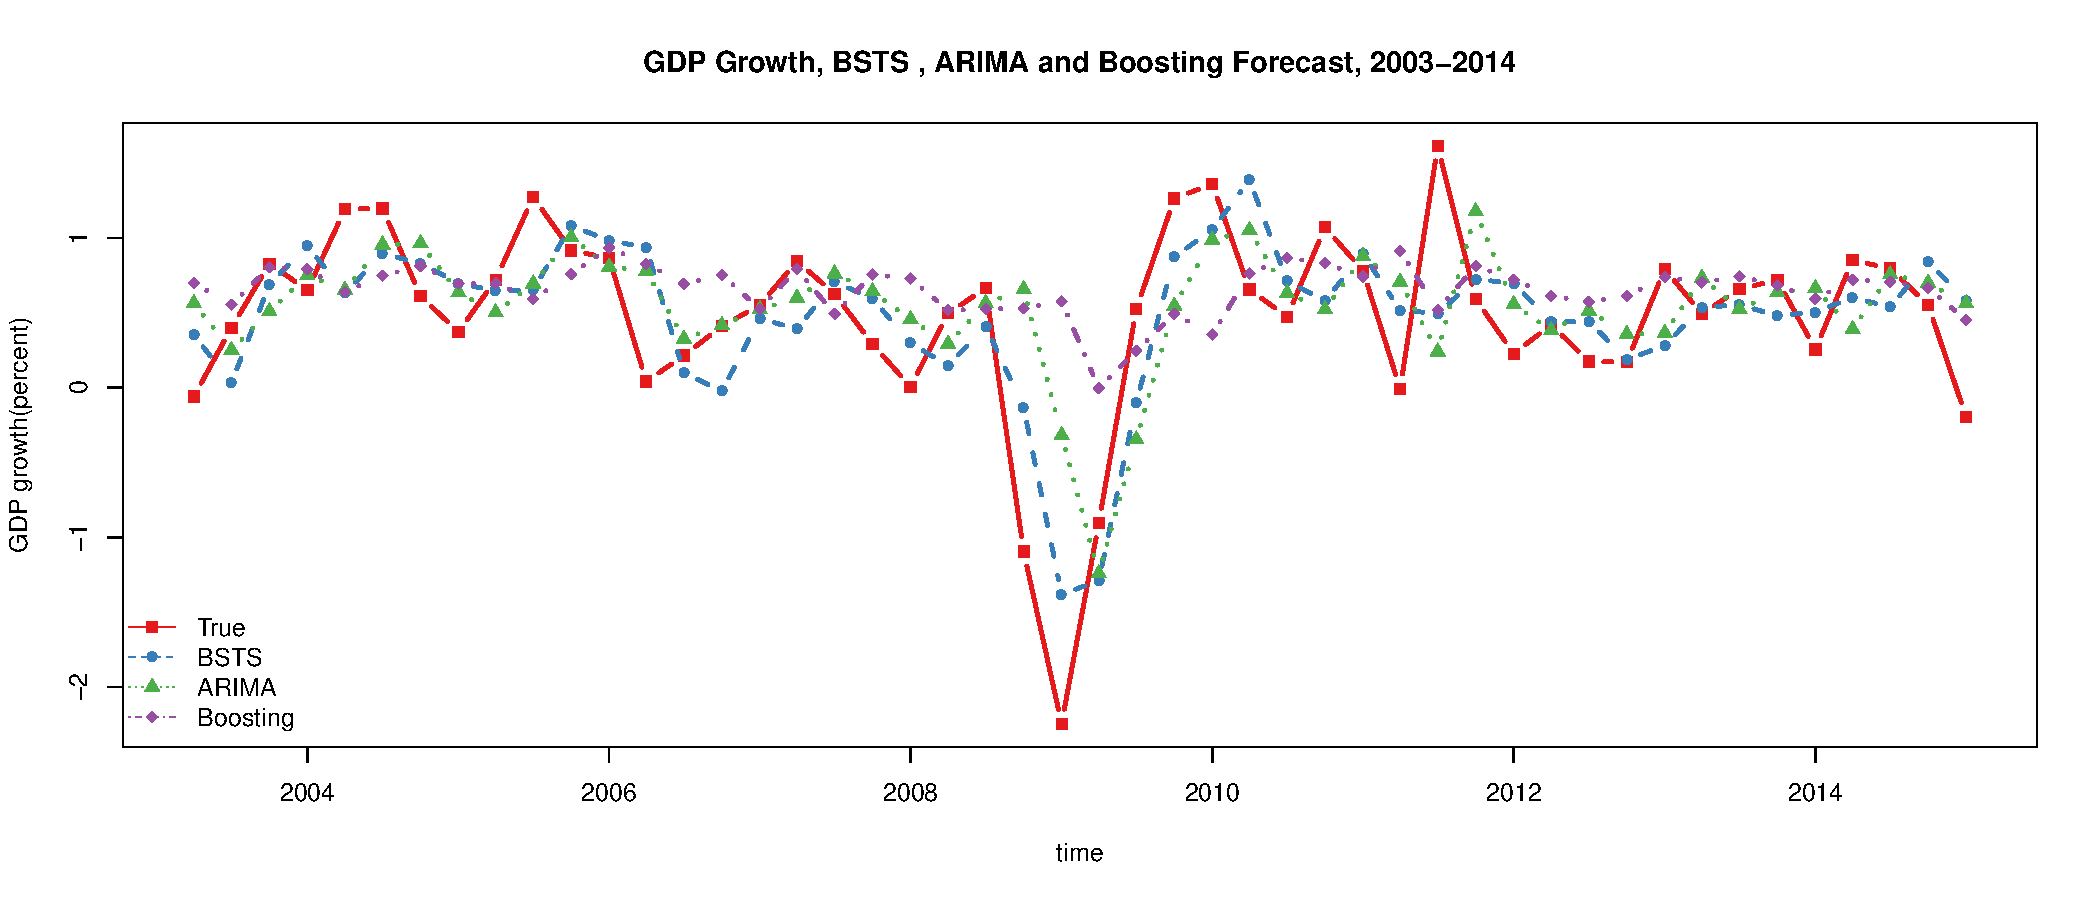
\includegraphics[width=1\linewidth]{Figures/bsts_arima_boost}
	\caption{GDP Growth, BSTS, ARIMA and Boosting Forecasts 2003-2015 }
	\label{fig:comparison}
\end{figure}


Figure ~\ref{fig:comparison} shows that the forecasts are very similar except during the 2008 to 2009 financial crisis. The one step ahead forecasts of ARIMA look like first order lag of target time series. The one step ahead forecasts of Boosting are very stable and look more like smoothed target time series. The one step ahead forecasts of BSTS are more volatile and do a  better job at capturing the  structural break during the 2008 to 2009 financial crisis. As we mentioned before, the signal among those leading predictors helps BSTS to predict the economic force which drives dramatic change in the target time series. 

We also calculate the forecast error in terms of the level of GDP. Table ~\ref{ErrorCom} shows that BSTS model is slightly better than  ARIMA and the Boosting model according to the regular criteria. 


% Please add the following required packages to your document preamble:
% \usepackage{booktabs}
\begin{table}[h]
	\centering
	\begin{tabular}{@{}llllll@{}}
		\toprule
					  & ME   & RMSE    & MAE     & MPE     & MAPE     \\ \midrule
		BSTS         & -159.853 & 6952.102 & 5641.339 & -0.008 & 0.356 \\
		ARIMA         & -1089.482 & 8996.830 & 6347.325 & -0.067 & 0.401  \\ 
		Boosting      & -792.281 &  8843.832 &  6349.097 &  -0.049 &  0.405\\ \bottomrule
	\end{tabular}
	\caption{Comparison of forecast error 2003-2015}
	\label{ErrorCom}
\end{table}

We also conduct the Diebold-Mariano test in which BSTS vs. ARIMA with the null hypothesis that the two methods have the same forecast accuracy and alternative hypothesis that ARIMA is less accurate than BSTS. The p-value is 0.061. We fail to reject the null hypothesis at the 5\% significance level. Similarly, we conduct the Diebold-Mariano Test in which BSTS vs. Boosting with the null hypothesis that the two methods have the same forecast accuracy and alternative hypothesis that Boosting is less accurate than BSTS. The p-value is 0.084. We fail to reject null hypothesis at the  5\%  significance level. In both cases, at the 10\% significance level, we will reject null hypothesis in favor of the alternatives that the forecasts of the ARIMA and Boosting models are  less accurate than forecasts of the BSTS model.


In order to inquire as to the performance of the three models in different scenarios, we separate the forecast horizon into three periods. We call the first period 2003 - 2007 the pre-crisis period; second period 2007-2011 the crisis period; and third period  2011-2015 the post-crisis period. The evidence shows that the performances of these three methods change during those periods.




\subsection{Comparison of one step ahead forecasts, 2003 to 2007}

During 2003 to 2007, the ARIMA model outperforms the other models. In Table ~\ref{ErrorCom1}, we can see that the performances of BSTS and Boosting are very close. 


\begin{table}[h]
	\centering
	\begin{tabular}{@{}llllll@{}}
		\toprule
				   & ME    & RMSE   & MAE  & MPE & MAPE     \\ \midrule
		BSTS       & 228.032 & 5748.218 & 4713.560 & 0.016 & 0.318 \\
		ARIMA      & -163.452 & 5199.532 & 4023.557 &-0.010 & 0.273  \\ 
		Boosting   & -1263.461 & 6078.649 & 4748.083 & -0.084 & 0.320\\ \bottomrule
	\end{tabular}
	\caption{Comparison of forecast error 2003-2007}
	\label{ErrorCom1}
\end{table}




\begin{figure}[h]
\centering
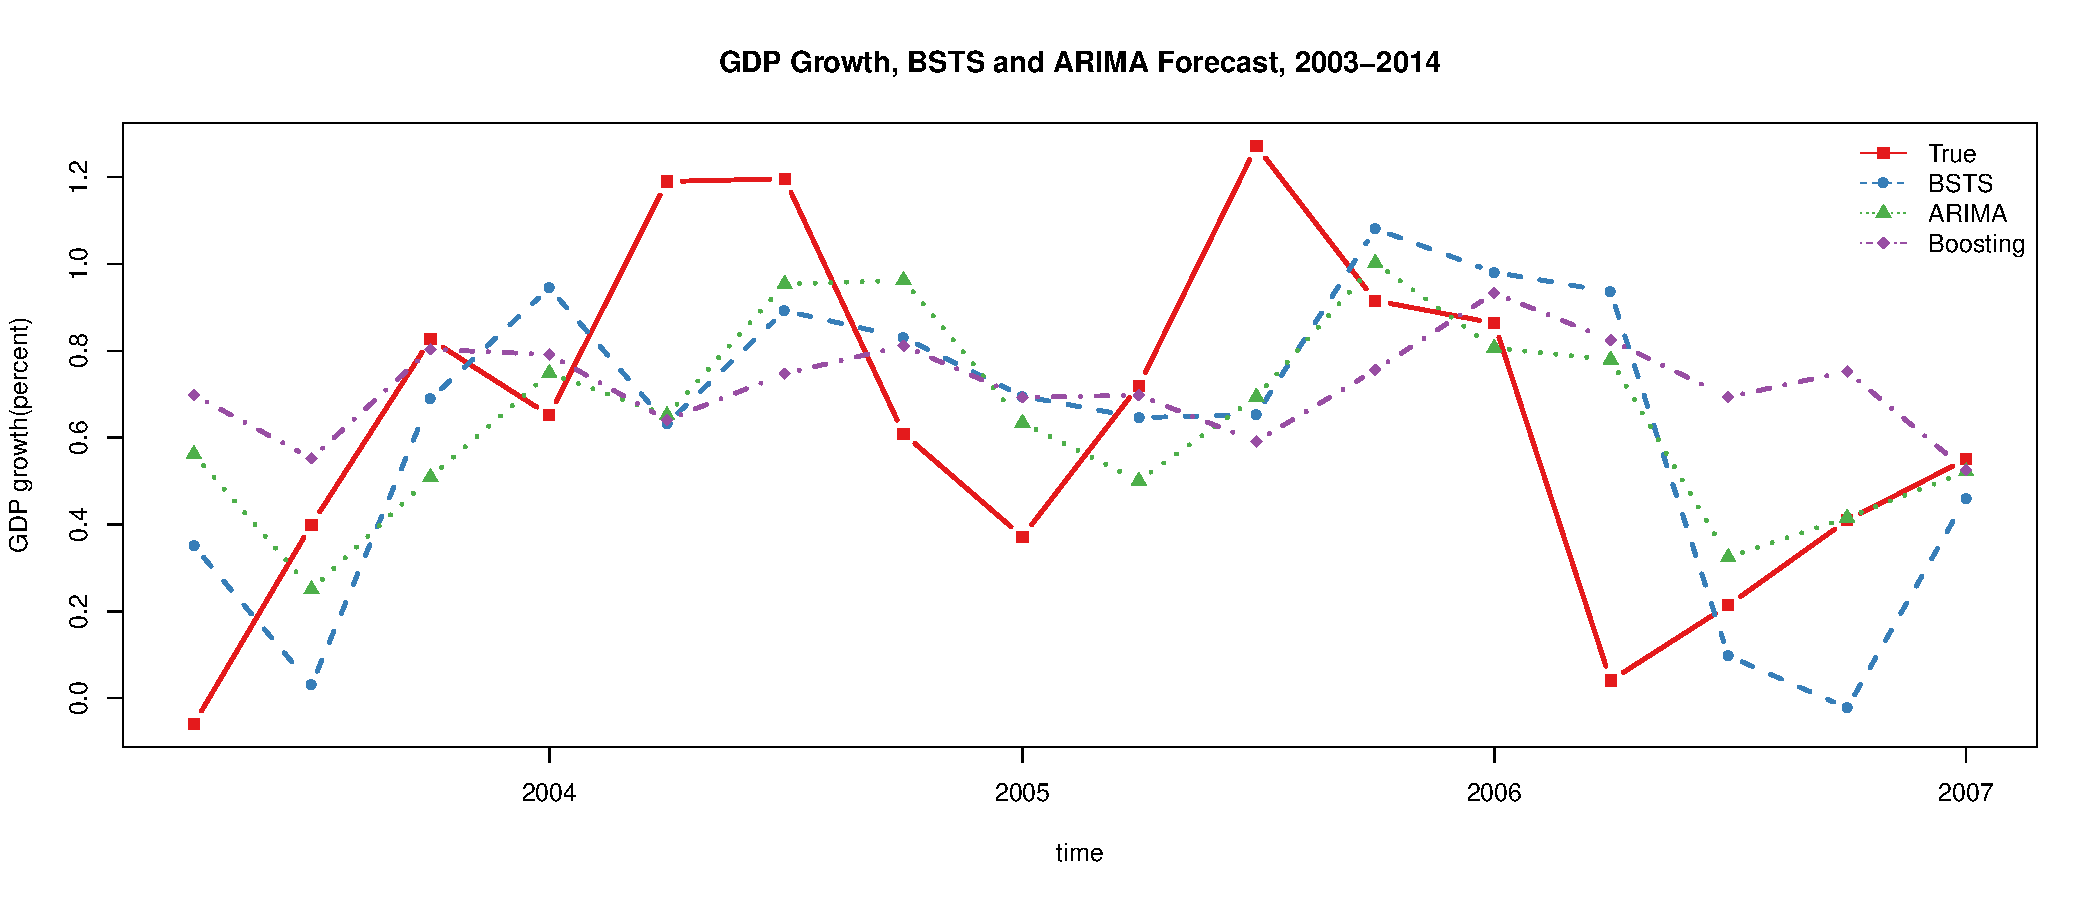
\includegraphics[width=0.9\linewidth]{Figures/bsts_arima_boost_1}
\caption{GDP Growth, BSTS, ARIMA and Boosting Forecast, 2003-2007}
\label{fig:bsts_arima_boost_1}
\end{figure}


Figure ~\ref{fig:bsts_arima_boost_1} shows that the ARIMA model outperforms the other two models. The BSTS model does not show anyadvantage over ARIMA 

 \subsection{Comparison of one step ahead forecasts, 2007 to 2011}
 
During the crisis period, BSTS performs much better than ARIMA and Boosting. It confirms  \citeA{Petris2008}'s statement that a state-space model can capture the structural break or change point better than an ARIMA model. 

\begin{table}[h]
	\centering
	\begin{tabular}{@{}llllll@{}}
		\toprule
				& ME     & RMSE   & MAE   & MPE  & MAPE   \\ \midrule
		BSTS    &  -384.114 & 7754.361 & 6719.998 & -0.023 & 0.427 \\
		ARIMA   & -1909.907 & 12000.140 & 8508.274 & -0.121 & 0.543 \\ 
		Boosting& -4373.490 & 14798.320 & 9544.599 & -0.281 & 0.610\\ \bottomrule
	\end{tabular}
	\caption{Comparison of forecast error 2007-2011}
	\label{ErrorCom2}
\end{table}

During 2007 to 2011, the financial crisis hindered economic development in many ways, Canadian GDP plunged as did other countries' GDP. In Figure ~\ref{fig:bsts_arima_boost2}, the ARIMA and Boosting models detect the decreasing in GDP later than BSTS. BSTS does not only use a state-space model to capture the dynamics of GDP, but also gets the signal of the structural change from the leading predictor such as stock market return or unemployment rate.  

\begin{figure}[h]
\centering
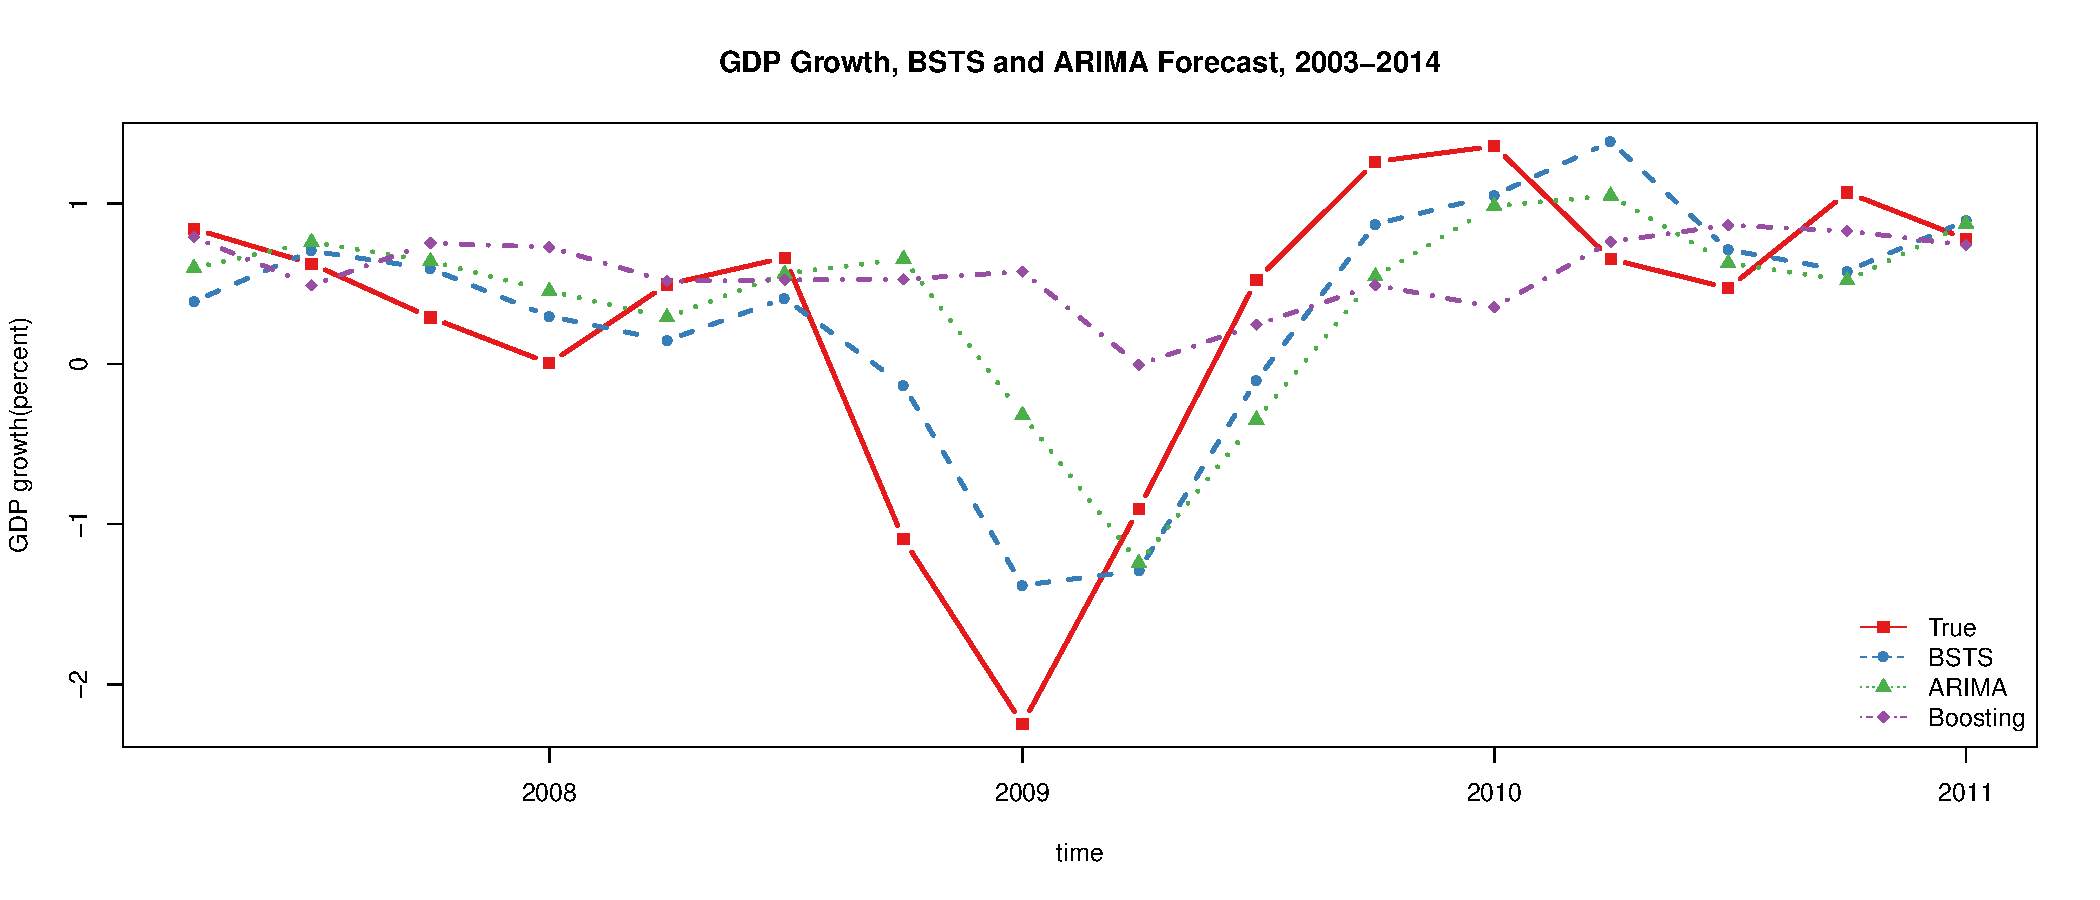
\includegraphics[width=0.9\linewidth]{Figures/bsts_arima_boost_2}
\caption{GDP Growth, BSTS, ARIMA and Boosting Forecasts, 2007-2011}
\label{fig:bsts_arima_boost2}
\end{figure}

Figure ~\ref{fig:bsts_arima_boost2} shows that the BSTS model outperforms other two models. Especially, during 2008, the GDP growth rate decreases abruptly, but ARIMA and Boosting models still predict GDP will keep stable. Only BSTS model forecasts the direction of change in GDP growth rate correctly,  and the forecasted magnitude of the change in GDP growth rate is close to the true value as well.  



\subsection{Comparison of one step ahead forecasts, 2011 to 2015}


During 2011 to 2015, the ARIMA model performs a little worse than the BSTS and Boosting models. Table ~\ref{ErrorCom3} shows that the performance of BSTS just is a little better than the Boosting model. 


\begin{table}[h]
	\centering
	\begin{tabular}{@{}llllll@{}}
		\toprule
		             & ME          & RMSE      & MAE       & MPE       & MAPE     \\ \midrule
		BSTS          & -321.159 & 7198.822 & 5490.460 & -0.017 & 0.324 \\
		ARIMA         & -1195.086 & 8472.912 & 6510.144 & -0.069 & 0.385 \\ 
		Boosting      & -2773.160 & 7512.228 & 5656.435 & -0.164 & 0.336\\ \bottomrule
	\end{tabular}
	\caption{Comparison of forecast error 2011-2015}
	\label{ErrorCom3}
\end{table}

Figure ~\ref{fig:bsts_arima_boost_3} shows that the forecast of ARIMA model is more like a first order lag of the target variable. The ARIMA model shows this pattern during the whole test period. The forecast of THE BSTS model is more volatile than during 2003 to 2007, and its dynamics are closer to the dynamics of the target variable. The forecast of the Boosting model is more steady as it does in entire test period. 

\begin{figure}[h]
	\centering
	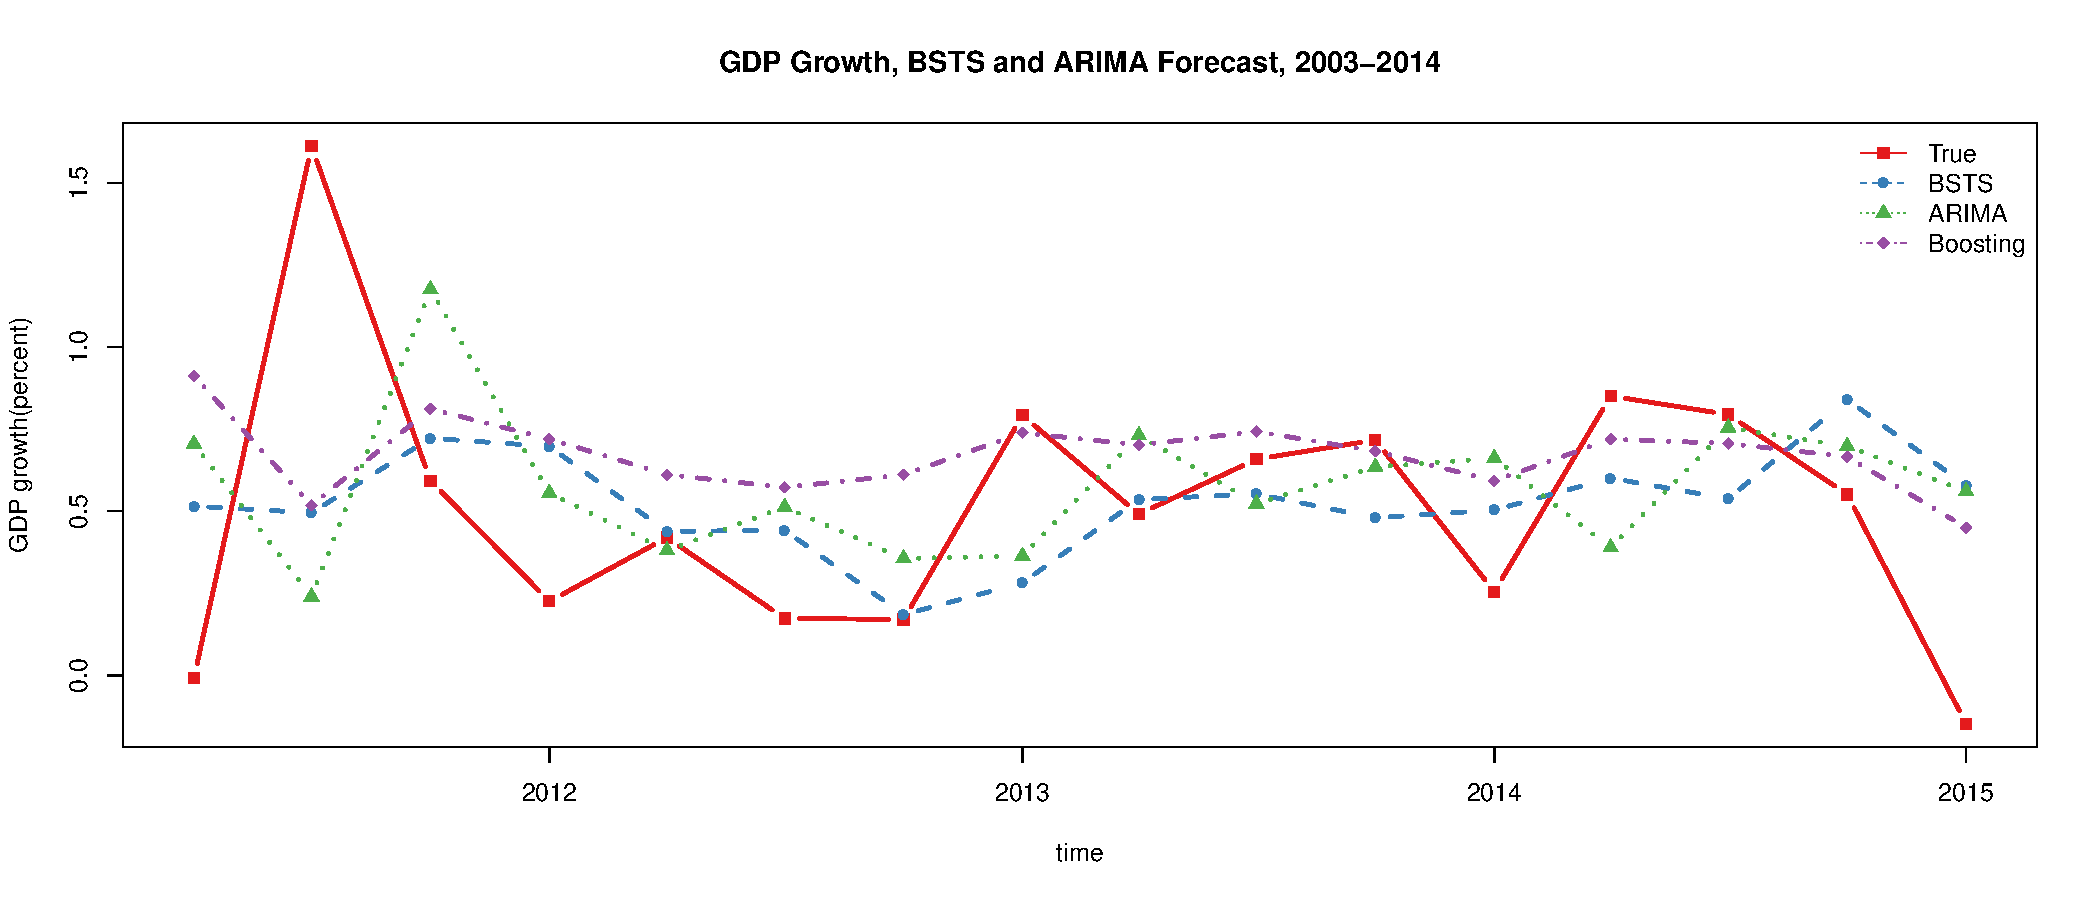
\includegraphics[width=0.9\linewidth]{Figures/bsts_arima_boost_3}
	\caption{GDP Growth, BSTS, ARIMA and Boosting Forecasts, 2011-2015}
	\label{fig:bsts_arima_boost_3}
\end{figure}



The performances of the three model change during the three different test periods. ARIMA does best in the first period and worst in the last period. BSTS does best in crisis period. Boosting does worst in the first period and does well in the last period. One potential reason is that including more data in the model when the time dimension expands helps improve the performance of BSTS and the Boosting model. The Boosting model ensembles many weak classifiers and is robust to over-fitting. Based on similar reasons, the BSTS model is getting better in the last test period. The ARIMA model is a univariate model, and when the time coverage extends, the increase in number of data points is very limited. Then the performance improves very slowly.
    






	


